\documentclass[10pt]{beamer}

\usetheme{metropolis}

\usepackage{booktabs}
\usepackage{array}
\usepackage[utf8]{inputenc}
\usepackage{pgfplots}
\usepackage{stmaryrd}
\usepackage{mathrsfs}
\usepackage{amsmath}
\usepackage{stmaryrd}
\usepackage{amsfonts}
\usepackage{movie15}
\usepackage{amssymb}
\usepackage{accsupp}
\usepackage{amsthm}
\usepackage{verbatim,cprotect}
\usepackage{listings}
\usepackage{hyperref}
\usepackage{enumerate}
\usepackage{tikz}
\usepackage[percent]{overpic}
\usepackage{tcolorbox}
\usepackage{color}
\usepackage{xspace}
\usepackage{alltt}
\usepackage{flushend}
\usepackage{graphicx}
\usepackage{wrapfig}
\usepackage[underline=false]{pgf-umlsd}

\usepackage[portuguese]{babel}
\usepackage[utf8]{inputenc}  % for proper diacritics
\usepackage[T1]{fontenc}
\usepackage {listings}
\usepackage{tikz}
% \usepackage{xcolor}
% Links
\usepackage{hyperref}

\usepackage{amsmath,amssymb}
%\usepackage{stmaryrd}
\usepackage{listings,color}
\usepackage{alltt}
\usepackage{flushend}



%\usepackage[T1]{fontenc}

% \lstdefinestyle{Go}{	
% 	keywordstyle=[1]\bfseries,
% 	basicstyle=\footnotesize\ttfamily,	
% 	numberstyle=\tiny,
% 	numbersep=5pt,
% 	breaklines=true,
% 	%prebreak=\raisebox{0ex}[0ex2][0ex]{\ensuremath{\hookleftarrow}},
% 	showstringspaces=false,
% 	upquote=true,
% 	tabsize=3,
% 	frame=tb,
% 	morekeywords={go,make,chan,int,import,main,func,for,select,case,string},
%       }

\lstdefinelanguage{Golang}%
  {morekeywords=[1]{package,import,func,type,struct,return,defer,panic,%
     recover,select,var,const,iota,},%
   morekeywords=[2]{string,uint,uint8,uint16,uint32,uint64,int,int8,int16,%
     int32,int64,bool,float32,float64,complex64,complex128,byte,rune,uintptr,%
     error,interface},%
   morekeywords=[3]{map,slice,make,new,nil,len,cap,copy,close,true,false,%
     delete,append,real,imag,complex,chan,},%
   morekeywords=[4]{for,break,continue,range,goto,switch,case,fallthrough,if,%
     else,default,},%
   morekeywords=[5]{Println,Printf,Error,Print,},%
   sensitive=true,%
   morecomment=[l]{//},%
   morecomment=[s]{/*}{*/},%
   morestring=[b]',%
   morestring=[b]",%
   morestring=[s]{`}{`},%
}

      
\lstdefinelanguage{SePi}%
  {morekeywords=[1]{type,integer,string,boolean,new, select, assume, assert},%
   sensitive=true,%
   morecomment=[l]{//},%
   morecomment=[s]{/*}{*/},%
   morestring=[b]',%
   morestring=[b]",%
   morestring=[s]{`}{`},%
 }

\lstdefinelanguage{CFST}%
{
  morekeywords=[1]{Int, Char, Bool, Skip, forall, rec, let, in, if, then, else, new, send, receive,
    select, fork, case, of, data, match, with},%  
  sensitive=true,%
  literate={->}{{$\rightarrow$}}1,%
   breaklines=true,
   morecomment=[l]{--},%
   morecomment=[s]{{-}{-}},%
   morestring=[b]',%
   morestring=[b]",%
   morestring=[s]{`}{`},%
 }

 

% notes
\newcommand{\todo}[1]{[{\color{blue}\textbf{#1}}]}

% Keywords
\newcommand{\keyword}[1]{\mathsf{#1}}

% Prekinds

\newcommand\prekind{\upsilon}

\newcommand{\stypes}{\mathcal S}
\newcommand\kinds{\stypes}

\newcommand{\types}{\mathcal T}
\newcommand\kindt{\types}

\newcommand\kindsch{\mathcal C}

% Multiplicity
\newcommand\Un{\ensuremath{\mathbf{u}}} % \infty
\newcommand\Lin{\ensuremath{\mathbf{l}}} % 1 

% Kinds
\newcommand\kind{\kappa}

% Grammars
\newcommand{\grmeq}{\; ::= \;}
\newcommand{\grmor}{\;\mid\;}

% type constructors
\newcommand\tcBase{B}
\newcommand\tcLolli\multimap
\newcommand\tcFun\to
\newcommand\tcBang{\mathop!}

% Keywords for types
\newcommand\kRec{\keyword{rec}}


% Types
\newcommand{\tskip}{\keyword{Skip}}
\newcommand\tSemi[2]{#1;#2}
\newcommand\tOut[1]{\tcBang#1}
\newcommand\tIn[1]{?#1}
\newcommand\tIChoice[1]{\oplus#1}
\newcommand\tEChoice[1]{\&#1}
\newcommand\tUnFun[2]{#1\tcFun#2}
\newcommand\tLinFun[2]{#1\tcLolli#2}
\newcommand\tPair[2]{#1\otimes#2}
\newcommand\tDatatype[1]{{[#1]}}
\newcommand\tRec[2]{\mu\,#1\,.\,#2}
\newcommand\tForall[2]{\forall\,#1\,.\,#2}

\newcommand\tRecK[2]{\kRec\,#1\,.\,#2}
% Environments
% \newcommand\emptyEnv{\cdot}
\newcommand\emptyEnv{\varepsilon}
\newcommand\kindEnv{\Delta}
\newcommand\varEnv{\Gamma}

% Language
% Expressions
% Language Types
\newcommand{\unite}{\keyword{Unit}}
\newcommand{\inte}{\keyword{Int}}
\newcommand{\chare}{\keyword{Char}}
\newcommand{\boole}{\keyword{Bool}}

% Variables
\newcommand\vare[1]{#1}
\newcommand\unlete[3]{\keyword{let} \; #1 = #2 \; \keyword{in} \; #3} 

% Applications
\newcommand\appe[2]{#1#2}
\newcommand\tappe[2]{#1[#2]}

% Conditional
\newcommand\conditionale[3]{\keyword{if}\;#1\;\keyword{then}\;#2\;\keyword{else} \; #3}

% Pairs
\newcommand\paire[2]{(#1,#2)}
\newcommand\binlete[4]{\keyword{let}\;#1, #2 = #3\;\keyword{in}\;#4}

% Session Types
\newcommand\newe[1]{\keyword{new}\;#1}
\newcommand\sende[2]{\keyword{send}\;#1\; #2}
\newcommand\recve[1]{\keyword{receive}\;#1}
\newcommand\selecte[1]{\keyword{select}\;#1}
\newcommand\matche[2]{\keyword{match}\;#1\;\keyword{with}\;#2}

% Fork
\newcommand\forke[1]{\keyword{fork}\;#1}

% Datatypes
\newcommand{\ctrcte}{C}
\newcommand\casee[2]{\keyword{case}\;#1\;\keyword{of}\;#2}

% Goal
\newcommand\Alg{\vdash_{a}}

% Equivalent
\newcommand\Equiv[2]{#1\,\thicksim\,#2}


%%% Local Variables:
%%% mode: latex
%%% TeX-master: "cfst-inforum18"
%%% End:
      
%\lstset{identifierstyle=\color{identifierColor}}

\title[Deciding the bisimilarity of context-free session types]{Deciding the bisimilarity of context-free session types}

\date{
\vspace*{1cm}
\begin{center}
	March 2021
\end{center}}
\author[B.Almeida, A.Mordido, V.Vasconcelos]{\underline{Bernardo Almeida}, Andreia Mordido, and Vasco T. Vasconcelos}
\institute[LASIGE, Faculdade de Ci\^encias, ULisboa]{LASIGE, Faculdade de Ci\^encias, Universidade de Lisboa \\\\
}
%\titlegraphic{\hfill
\includegraphics[height=1.5cm]{logo.png}}

\begin{document}
\lstset{language=Haskell}

\maketitle

\begin{frame}[fragile]{Motivation}
\vspace*{5mm}

\begin{lstlisting}[language=CFST]
data Tree = Leaf | Node Int Tree Tree
\end{lstlisting}

\begin{lstlisting}[language=CFST]
sendTree Leaf c =
  select Leaf c
sendTree (Node x l r) c =
  let c1 = select Node c
      c2 = send x c1
      c3 = sendTree l c2
      c4 = sendTree r c3
   in c4
\end{lstlisting}
  
\vspace*{-1.8cm}
\hfill 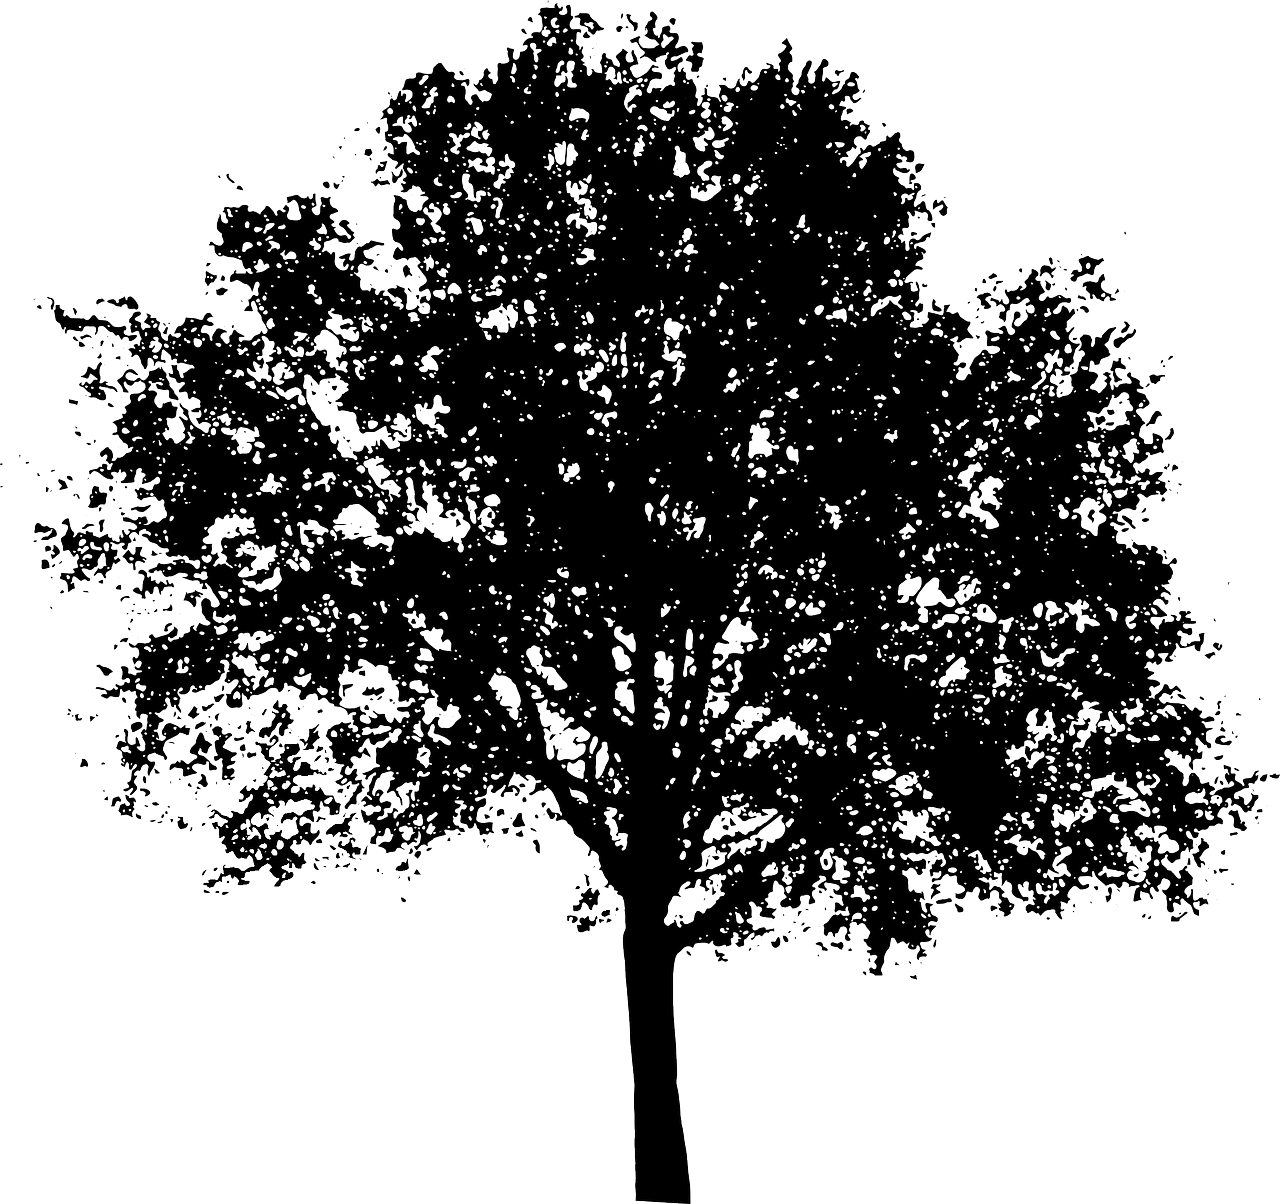
\includegraphics[height=4cm]{img/tree}
\end{frame}

\begin{frame}
  \frametitle{Context-Free Session Types}
  \begin{align*}
  S,T &\grmeq \skipk \grmor \sharp B \grmor 
  \star\{\ell_i\colon T_i\}_{i\in I} \grmor S;T \grmor \mu X.T \grmor X
  \\
  \sharp &\grmeq {}! \grmor {}? 
  \\
  \star  &\grmeq \oplus \grmor {}\&
  % \qquad \qquad
  % a \grmeq \sharp B \grmor \star l \grmor X
\end{align*}

\end{frame}

%\begin{frame}{Table of contents}
%    \frametitle{Layout}
%    \setbeamertemplate{section in toc}[sections numbered]
%  \tableofcontents[hideallsubsections]
%\end{frame}

% \begin{frame}{Plan}

%   	\metroset{block=fill}
%   	\begin{definition}[Type equivalence problem] 
%     	\smallskip 
%     	Given any context-free session types $S$ and $T$, the type equivalence problem consists in deciding if types $S$ and $T$ are equivalent, i.e., $S\sim T$.
%   	\end{definition}

%   	\begin{itemize}
%     	\item Implement an algorithm that decides the \emph{type equivalence problem}.
%     	\item Prove its soundness and completeness w.r.t.\ the metatheory of context-free session types proposed by Thiemann and Vasconcelos.
%     	\item Provide results on complexity.
%   	\end{itemize}
% \end{frame}

%\section{Algorithm for checking the equivalence of context-free session types}

\begin{frame}{Algorithm for checking the equivalence of CFST \hfill {\color{mLightBrown}Main stages}}
	\begin{center}
    	\begin{tikzpicture}[node distance = 2.5cm, auto]
      		% Place nodes
      		\node [block2] (typeToGrammar) {{\bf Convert types to a grammar}\\ Translates types into a (finite) set of productions}; 
      		\node [block2,below=5mm of typeToGrammar] (prune) {{\bf Prune unnormed productions}\\ Streamlines the grammar by pruning unnormed productions};%
      		\node [block2,below=5mm of prune] (simplifyExpand) {{\bf Simplify and expand}\\ Alternates between simplification and expansion operations, until reaching a successful branch in the expansion tree or concluding that all branches are unsuccessful };
      		% Draw edges
      		\path [line] (typeToGrammar) -- (prune);
      		\path [line] (prune) -- (simplifyExpand);
   		\end{tikzpicture}
  	\end{center}
\end{frame}


\begin{frame}{Convert types to a grammar}
  
  	\vspace*{-1cm}
  	\hspace*{-3mm}\parbox{8cm}{
  	\vspace*{-2.5cm}
  	  	We consider a finite set of productions $X \rightarrow a \vec Y$ where:
   	\begin{itemize}
     	\item $X, Y$ represent \emph{non-terminal symbols}
     	\item $a$ is a \emph{terminal symbol} (a \emph{label} in the labelled transition system)
   	\end{itemize}
	}\hfill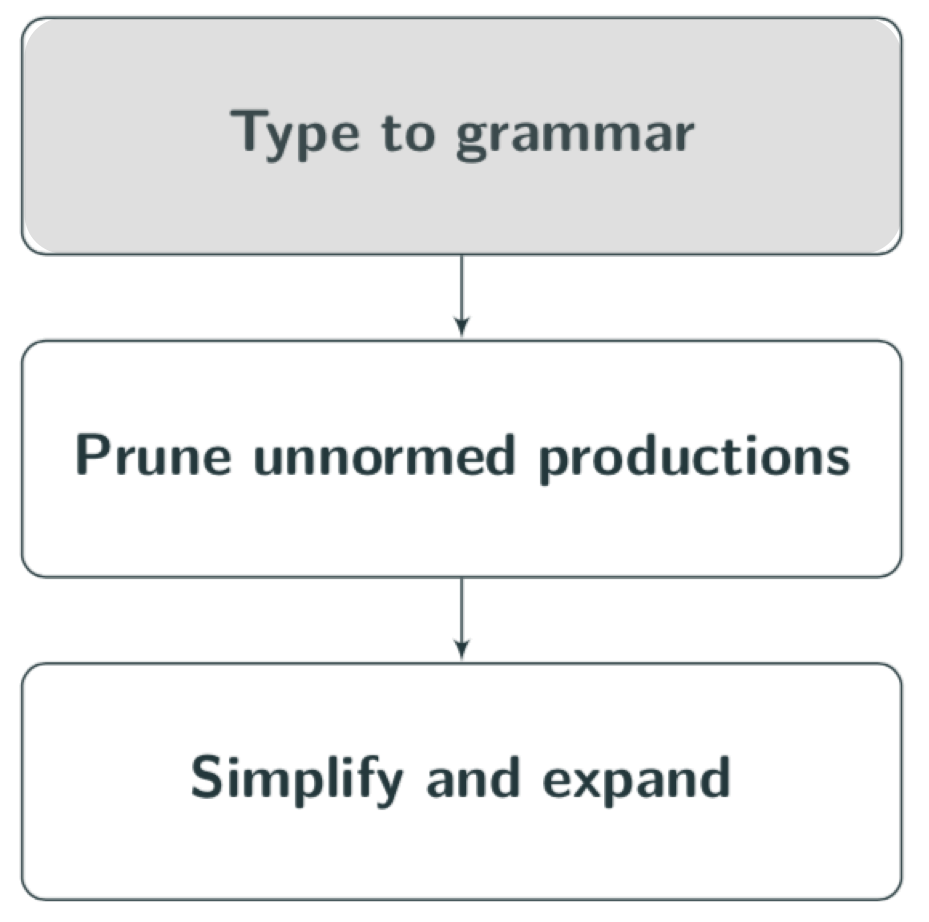
\includegraphics[height=2.8cm]{img/typeToGrammar.png}
	Context-free session types are seen as \emph{simple grammars}:
  	\begin{itemize}
		\item context-free grammars in \emph{Greibach normal form} 
		\item s.t. for each $X$ and $a$ there is at most one production $X \rightarrow a \vec Y$
  	\end{itemize}
\end{frame}


\begin{frame}{Convert types to a grammar}

  	\hfill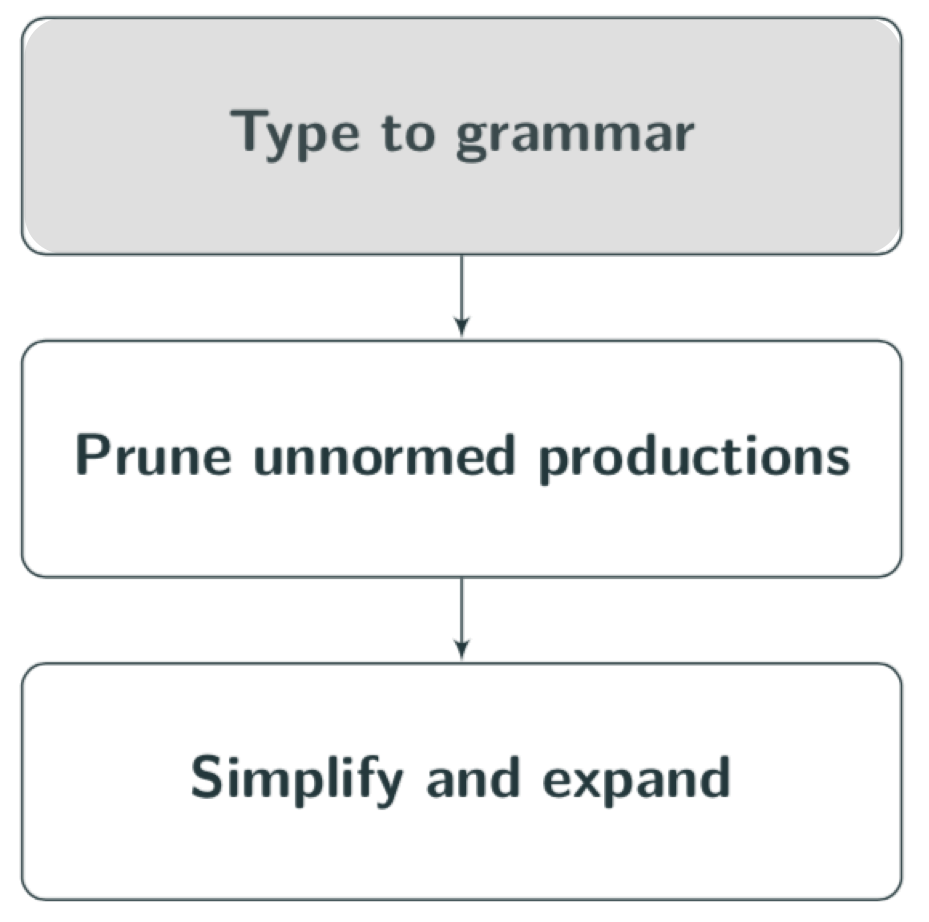
\includegraphics[height=2.8cm]{img/typeToGrammar.png}

  	\vspace*{-3cm}
  	{\color{teal} Example} \\
  
  	\begin{tabular} {l l }
    %   $S$ & $\triangleq (\mu X_1. \&\{n: X_1;X_1;?\intk, \ell: ?\intk\});(\mu X_2. !\intk ; X_2;X_2)$\\\smallskip 
    % $T$ & $\triangleq (\mu Y_1. \&\{n: Y_1;Y_1, \ell: \skipk\};?\intk);(\mu Y_2. !\intk ; Y_2)$
  		$S$ &$\triangleq (\mu x. \&\{n\colon x;x;?\,\intk,
      \ell\colon ?\,\intk \});( \mu z. !\,\intk; z;z )$\\\smallskip  
        $T$ &$\triangleq (\mu y. \&\{n\colon y;y,
      \ell\colon \skipk \}; ?\,\intk); (\mu z. !\,\intk; z)$\\
  	\end{tabular}
  
  	\pause \vspace*{5mm}
  	\begin{tabular}{l l l |l l l}
    	&Productions for $S$& & & Productions for $T$& \\ \hline
    	&\uncover<3-> {{\color{gray}$X_{} \rightarrow \,! (\,)\,X_1 X_4$}} & & &\uncover<3-> {{\color{gray}$Y_{} \rightarrow \,! (\,)\, Y_1 Y_3 $} }&\\
    	&$X_1 \rightarrow \& n\, X_1 X_1 X_2$ & & &$Y_1 \rightarrow \& n\, Y_1 Y_1 Y_2 $ &\\
    	&$X_1 \rightarrow \& \ell\, X_3$ &&& $Y_1 \rightarrow \& \ell \,Y_2 $&\\
    	&$X_2 \rightarrow \,? \intk$&&& $Y_2 \rightarrow \,? \intk$&\\
    	&$X_3 \rightarrow \,? \intk$&&& $Y_3 \rightarrow \,!\intk\, Y_3$&\\
    	&$X_4 \rightarrow \,!\intk\, X_4 X_4$ &&&&\\
  	\end{tabular}	
\end{frame}

\begin{frame}{Algorithm for checking the equivalence of CFST \hfill {\color{mLightBrown}Main stages}}

  	\begin{center}
    	\begin{tikzpicture}[node distance = 2.8cm, auto]
      		% Place nodes
      		\node [block2] (typeToGrammar) {{\bf Convert types to a grammar}\\ 
      		{\color{gray}\texttt{LOHaskellCode $\sim$ 100}}\\
      		Soundness {\color{olive}\checkmark}
      		\begin{enumerate}
    	 		\item Conversion of types into BPAs is sound\footnote{ Thiemann and Vasconcelos. Context-free session types. 2016.}.
    	 		\item Conversion of BPAs to Greibach Normal Form without altering the solution is sound\footnote{ Baeten et al. Decidability of bisimulation equivalence for process generating context-free languages.  1993.}.
      		\end{enumerate}
      		}; 
      		\node [block2, below=5mm of typeToGrammar] (prune) {{\bf Prune unnormed productions}};
      		\node [block2, below=5mm of prune] (simplifyExpand) {{\bf Simplify and expand} };
      		\path [line] (typeToGrammar) -- (prune);
      		\path [line] (prune) -- (simplifyExpand);
    	\end{tikzpicture}
  	\end{center}
\end{frame}

\begin{frame} {Prune unnormed productions}
	\hfill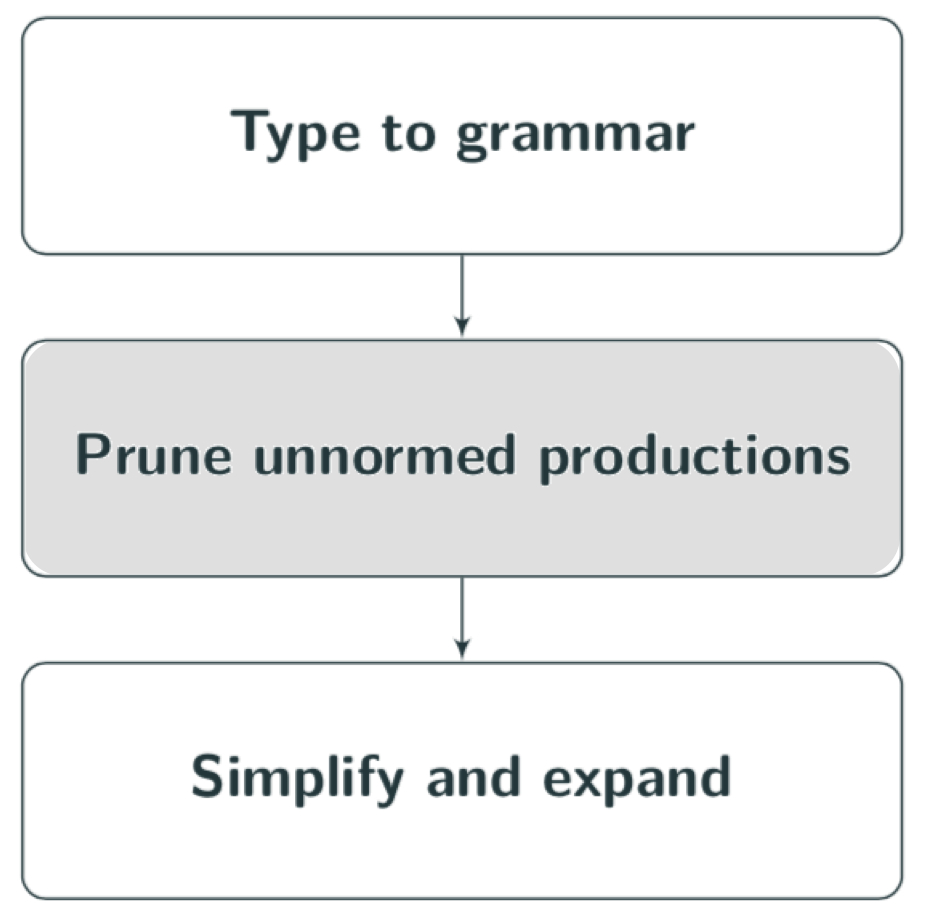
\includegraphics[height=2.8cm]{img/prune.png}

	\vspace*{-2.8cm}
	\metroset{block=fill}
	\begin{varblock}[7.8cm]{Definition ((Un)normed symbols)\footnote{\label{note1} Christensen et al. Bisimulation equivalence is decidable for all CF processes. 1995} }
			\smallskip 
		A sequence of symbols $\alpha$ is \emph{normed} if there is a path $\alpha \rightarrow \cdots \rightarrow \varepsilon$. 
		Otherwise, $\alpha$ is said to be \emph{unnormed}.\\
	\end{varblock}

	Christensen, Huttel, and Stirling\footnotemark[\value{footnote}] noted that:\\\smallskip
	\hspace*{1cm}	whenever $\alpha$ is unnormed, $\alpha \sim \alpha \beta$.

	\pause
	\vspace*{-1mm}
	{\color{teal}\rule{3cm}{2pt}}\\
   	{\color{teal} Example} \\\smallskip
	\vspace*{-7mm}

	$$S \triangleq (\mu x. \&\{n\colon x;x;?\,\intk,
      \ell\colon ?\,\intk \});( \mu z. !\,\intk; z;z )$$

	\vspace*{-2mm}
	\hspace*{5mm}\begin{tabular}{l l l }
 		&Productions for $S$&  \\ \hline
 	 	&$X_1 \rightarrow \& n\, X_1 X_1 X_2$ &\\
 	 	&$X_1 \rightarrow \& \ell\, X_3$ &\\
 	 	&$X_2 \rightarrow \,? \intk$&\\
 	 	&$X_3 \rightarrow \,? \intk$&\\
 	 	&$X_4 \rightarrow \,!\intk\, X_4 X_4$ &\\
	\end{tabular}
	\hspace*{1cm} \pause
	\begin{tabular}{l l l }
 		&Productions for \emph{pruned} $S$&  \\ \hline
  		&\hspace*{4mm}$X_1 \rightarrow \& n\, X_1 X_1 X_2$ & \\
  		&\hspace*{4mm}$X_1 \rightarrow \& \ell\, X_3$ &\\
 		&\hspace*{4mm}$X_2 \rightarrow \,? \intk$&\\
  		&\hspace*{4mm}$X_3 \rightarrow \,? \intk$&\\
  		&\hspace*{4mm}$X_4 \rightarrow \,!\intk\, X_4 $ &\\
	\end{tabular}
 	\vspace*{2mm}
\end{frame}


\begin{frame}{Algorithm for checking the equivalence of CFST \hfill {\color{mLightBrown}Main stages}}

	\begin{center}
		\begin{tikzpicture}[node distance = 2.8cm, auto]
   			% Place nodes
    		\node [block2] (typeToGrammar) {{\bf Convert types to a grammar}\\ 
    		{\color{gray}\texttt{LOHaskellCode $\sim$ 100}}\\
   			Soundness {\color{olive}\checkmark}
    		}; 
    		\node [block2, below=5mm of typeToGrammar] (prune) {{\bf Prune unnormed productions} \\ 
    		{\color{gray}\texttt{LOHaskellCode $\sim$ 30}}\\
    		Soundness {\color{olive}\checkmark} 
    		\begin{enumerate}
    			\item Pruning unnormed productions is sound\footnote{ Christensen, Huttel, and Stirling. Bisimulation equivalence is decidable for all \\ context-free processes. 1995}
    		\end{enumerate}
    		};
    		\node [block2, below=5mm of prune] (simplifyExpand) {{\bf Simplify and expand} };
    		% Draw edges
    		\path [line] (typeToGrammar) -- (prune);
    		\path [line] (prune) -- (simplifyExpand);
		\end{tikzpicture}
	\end{center}
\end{frame}


\begin{frame} {Simplify and expand}
	\hfill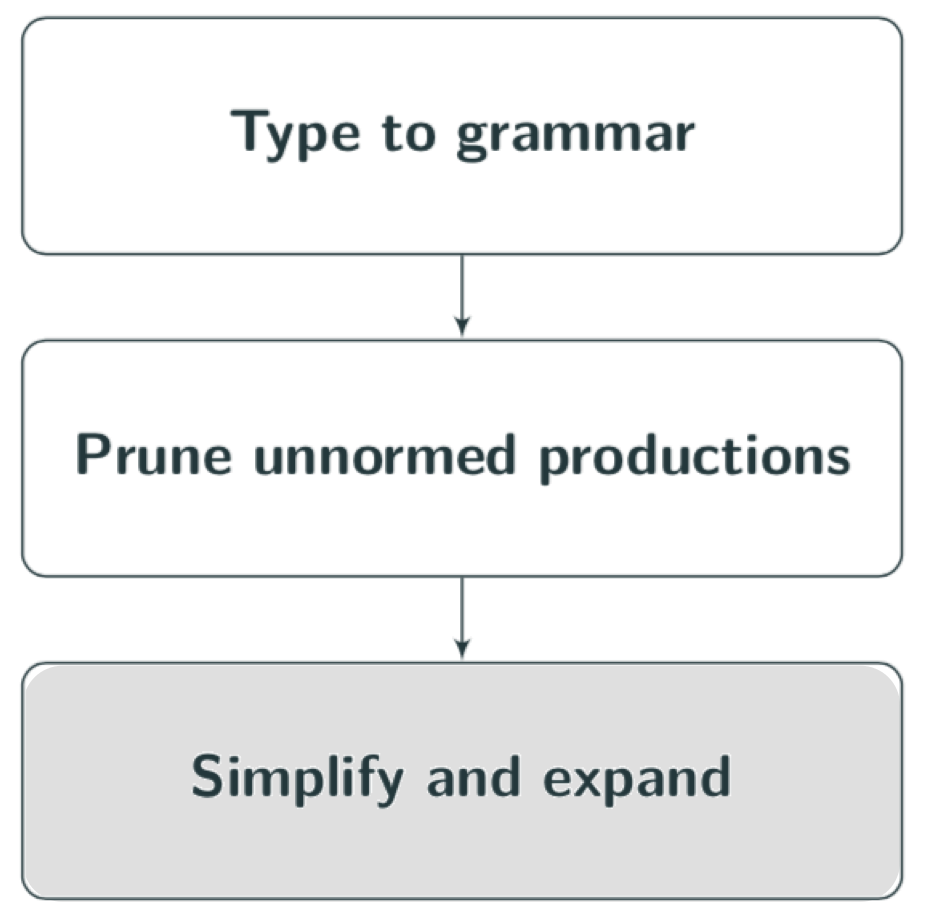
\includegraphics[height=2.8cm]{img/simplifyExpand.png}
	
	\vspace*{-3cm}
	Following the ideas from Hirshfeld, Jan{\v{c}}ar, Moller, \\
	a bisimulation is seen as an {\bf expansion tree}\footnote{Hirshfeld. Bisimulation trees and the decidability of weak bisimulations. 1997}\footnote{Jan{\v{c}}ar and Moller. Techniques for decidability and undecidability of bisimilarity. 1999}\\ that alternates between:
	\begin{itemize}
		\item { expansion operations}
		\item { simplification operations	}
	\end{itemize}
	\begin{center}
		\hspace*{-2mm}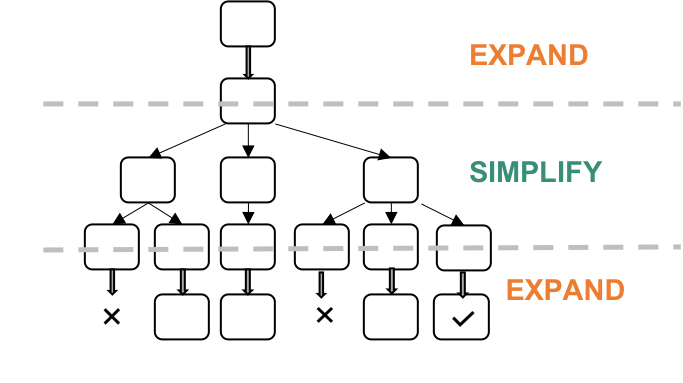
\includegraphics[height=4cm]{img/expand_simplify}
	\end{center}	
\end{frame}


\begin{frame} {Simplify and expand}
	An expansion tree alternates between:
	\vspace*{-1mm}
	\begin{itemize} 
		\item {\color{mLightBrown} \bf expansion operations} - a single derived node results from the expansion of the parent node. \pause
		\item {\color{teal}\bf simplification operations	}
		\begin{itemize}
			\item {\bf reflexive rule}: omit from a node $N$ any reflexive pair.
			\item {\bf congruence rule}: omit from a node $N$ any pair that belongs to the least congruence containing the ancestors of $N$. \pause
			\item {\bf basic process algebra rules}\footnote{Jan{\v{c}}ar, Moller. Techniques for decidability and undecidability of bisimilarity. 1999}\footnote{ Christensen et al. Bisimulation equivalence is decidable for all CF processes. 1995}\\
			\vspace*{-2mm}
			\hspace*{-2cm}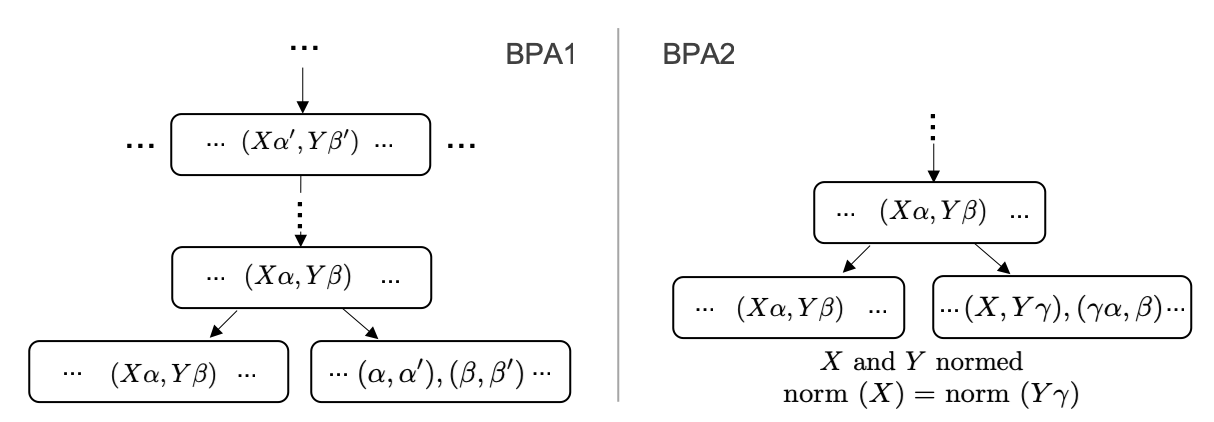
\includegraphics[height=4cm]{img/bpa_new}\smallskip
		\end{itemize}
	\end{itemize}
\end{frame}

\begin{frame}{Simplify and Expand}
	All these transformation rules preserve the \emph{safeness property}:
	\metroset{block=fill}
	\begin{block}{Safeness property\footnote{Jan{\v{c}}ar, Moller. Techniques for decidability and undecidability of bisimilarity. 1999}}
		\smallskip
		$S\sim T$ iff the expansion tree rooted at $\{(S,T\,)\}$ has a successful branch.	
	\end{block}
	
	The finite witness property holds\footnotemark[\value{footnote}]:
	
	\begin{block}{Finite witness property\footnotemark[\value{footnote}]\footnote{ Christensen et al. Bisimulation equivalence is decidable for all CF processes. 1995}}
		\smallskip
		If $S\sim T$, then there exists a {\bf finite successful branch} in the expansion tree.
	\end{block}
\end{frame}

\begin{frame}
	\begin{tabular} {l l l }
		{\color{teal}\rule{3cm}{2pt}} &  $S$ &$\triangleq (\mu x. \&\{n\colon x;x;?\,\intk,
     	 \ell\colon ?\,\intk \});( \mu z. !\,\intk; z;z )$\\
 		{\color{teal} Example}  &  $T$ &$\triangleq (\mu y. \&\{n\colon y;y,
     	 \ell\colon \skipk \}; ?\,\intk); (\mu z. !\,\intk; z)$
	\end{tabular}
	\vspace*{2mm}
	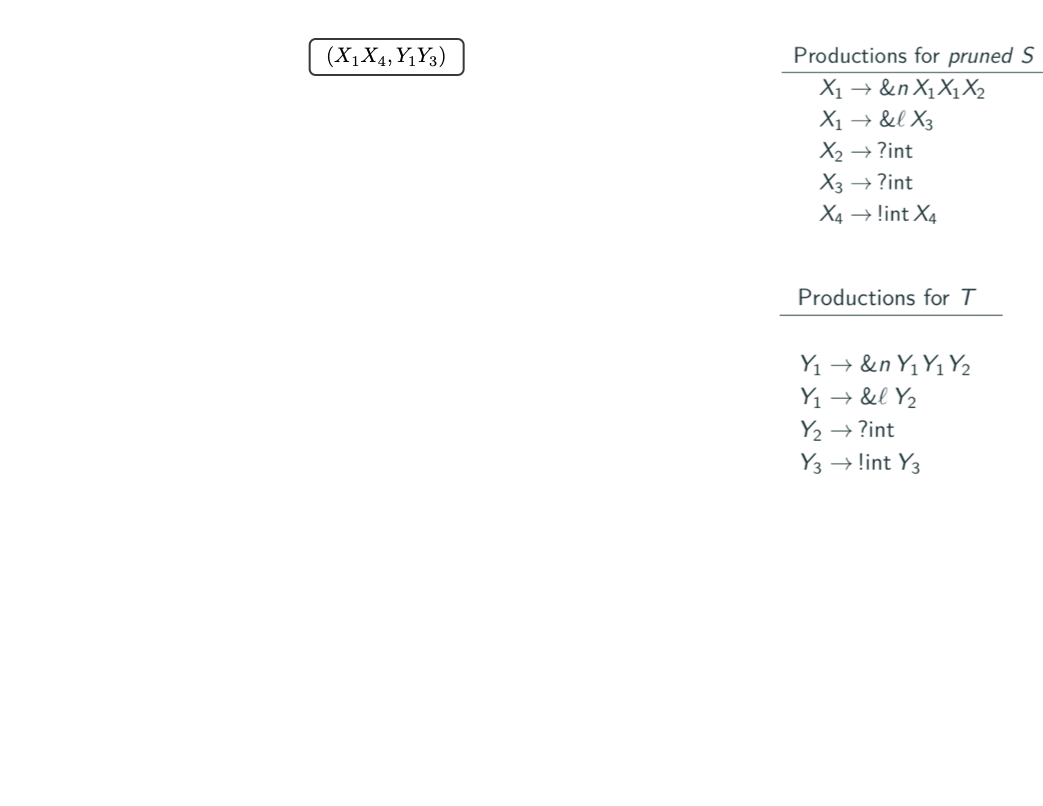
\includegraphics[width=11.5cm]{img/exemplo-9}\smallskip
\end{frame}

\begin{frame}
	\begin{tabular} {l l l }
  		{\color{teal}\rule{3cm}{2pt}} &  $S$ &$\triangleq (\mu x. \&\{n\colon x;x;?\,\intk,
      	\ell\colon ?\,\intk \});( \mu z. !\,\intk; z;z )$\\
  	{\color{teal} Example}  &  $T$ &$\triangleq (\mu y. \&\{n\colon y;y,
      \ell\colon \skipk \}; ?\,\intk); (\mu z. !\,\intk; z)$
	\end{tabular}
	\vspace*{2mm}
	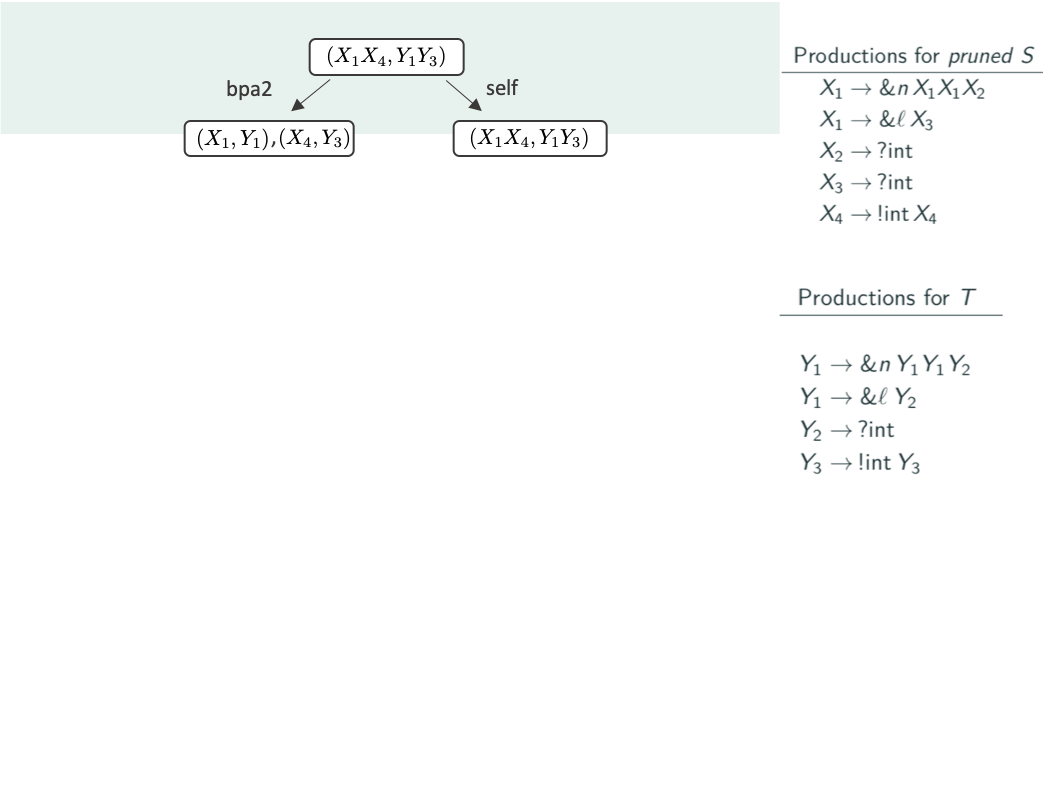
\includegraphics[width=11.5cm]{img/exemplo-8}\smallskip
\end{frame}


\begin{frame}
	\begin{tabular} {l l l }
  		{\color{teal}\rule{3cm}{2pt}} &  $S$ &$\triangleq (\mu x. \&\{n\colon x;x;?\,\intk,
      \ell\colon ?\,\intk \});( \mu z. !\,\intk; z;z )$\\
  		{\color{teal} Example}  &  $T$ &$\triangleq (\mu y. \&\{n\colon y;y,
      \ell\colon \skipk \}; ?\,\intk); (\mu z. !\,\intk; z)$
	\end{tabular}
	\vspace*{2mm}
	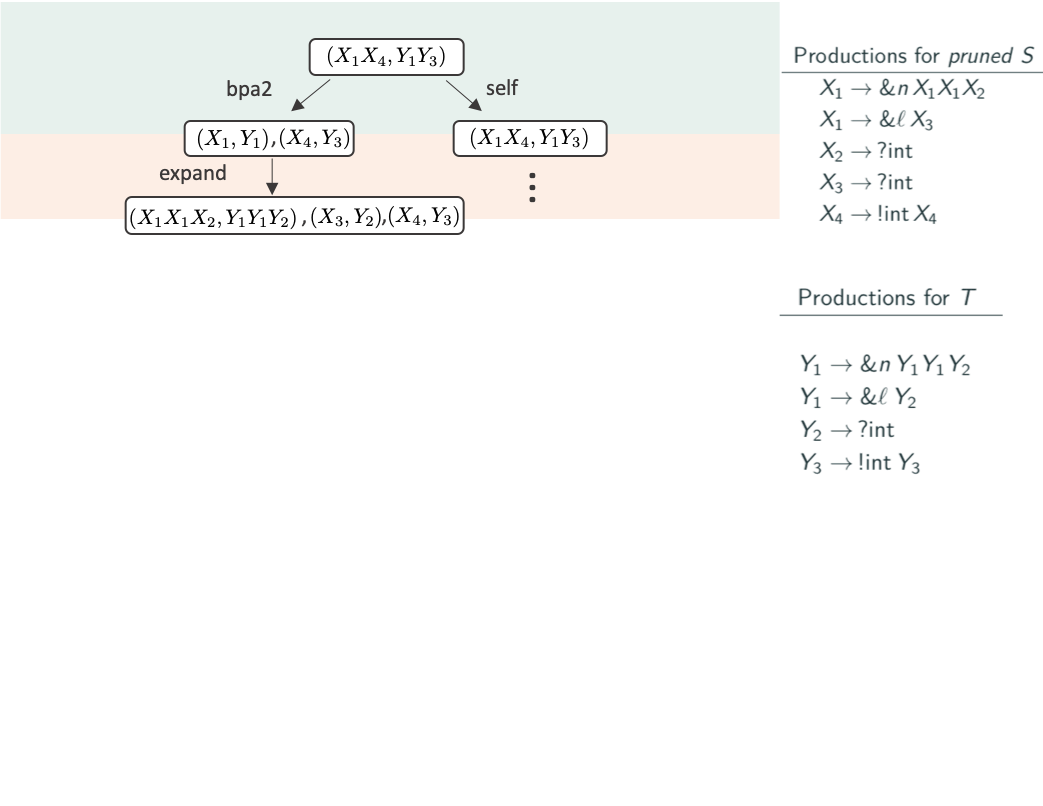
\includegraphics[width=11.5cm]{img/exemplo-7}\smallskip
\end{frame}

\begin{frame}
	\begin{tabular} {l l l }
  		{\color{teal}\rule{3cm}{2pt}} &  $S$ &$\triangleq (\mu x. \&\{n\colon x;x;?\,\intk,
      \ell\colon ?\,\intk \});( \mu z. !\,\intk; z;z )$\\
 		{\color{teal} Example}  &  $T$ &$\triangleq (\mu y. \&\{n\colon y;y,
      \ell\colon \skipk \}; ?\,\intk); (\mu z. !\,\intk; z)$
	\end{tabular}
	\vspace*{2mm}
	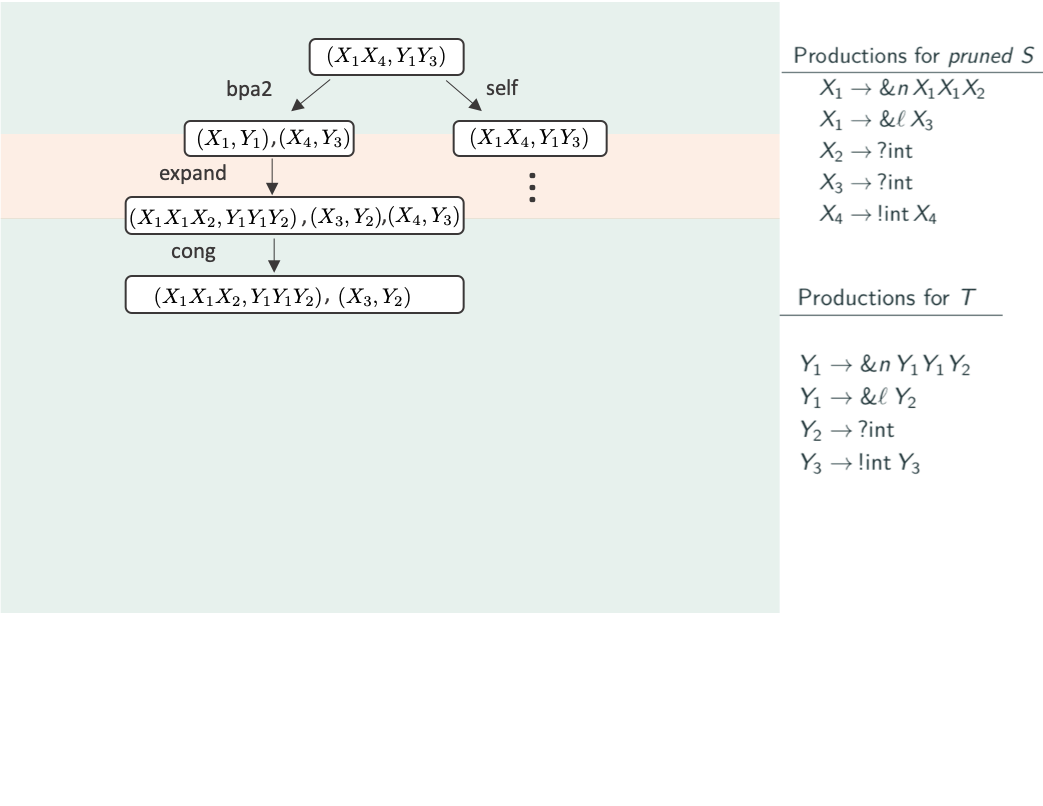
\includegraphics[width=11.5cm]{img/exemplo-6}\smallskip
\end{frame}

\begin{frame}
	\begin{tabular} {l l l }
  		{\color{teal}\rule{3cm}{2pt}} &  $S$ &$\triangleq (\mu x. \&\{n\colon x;x;?\,\intk,
      \ell\colon ?\,\intk \});( \mu z. !\,\intk; z;z )$\\
  		{\color{teal} Example}  &  $T$ &$\triangleq (\mu y. \&\{n\colon y;y,
      \ell\colon \skipk \}; ?\,\intk); (\mu z. !\,\intk; z)$
	\end{tabular}
	\vspace*{2mm}
	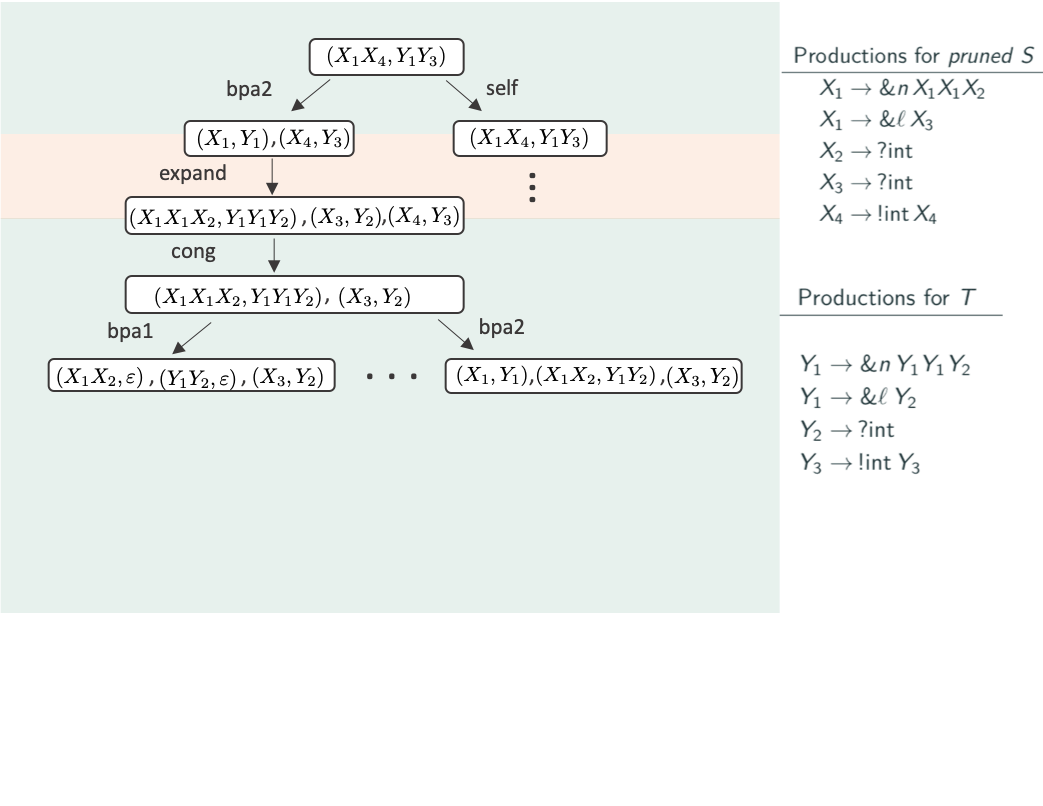
\includegraphics[width=11.5cm]{img/exemplo-5}\smallskip
\end{frame}

\begin{frame}
	\begin{tabular} {l l l }
  		{\color{teal}\rule{3cm}{2pt}} &  $S$ &$\triangleq (\mu x. \&\{n\colon x;x;?\,\intk,
      \ell\colon ?\,\intk \});( \mu z. !\,\intk; z;z )$\\
  		{\color{teal} Example}  &  $T$ &$\triangleq (\mu y. \&\{n\colon y;y,
      \ell\colon \skipk \}; ?\,\intk); (\mu z. !\,\intk; z)$
	\end{tabular}
	\vspace*{2mm}
	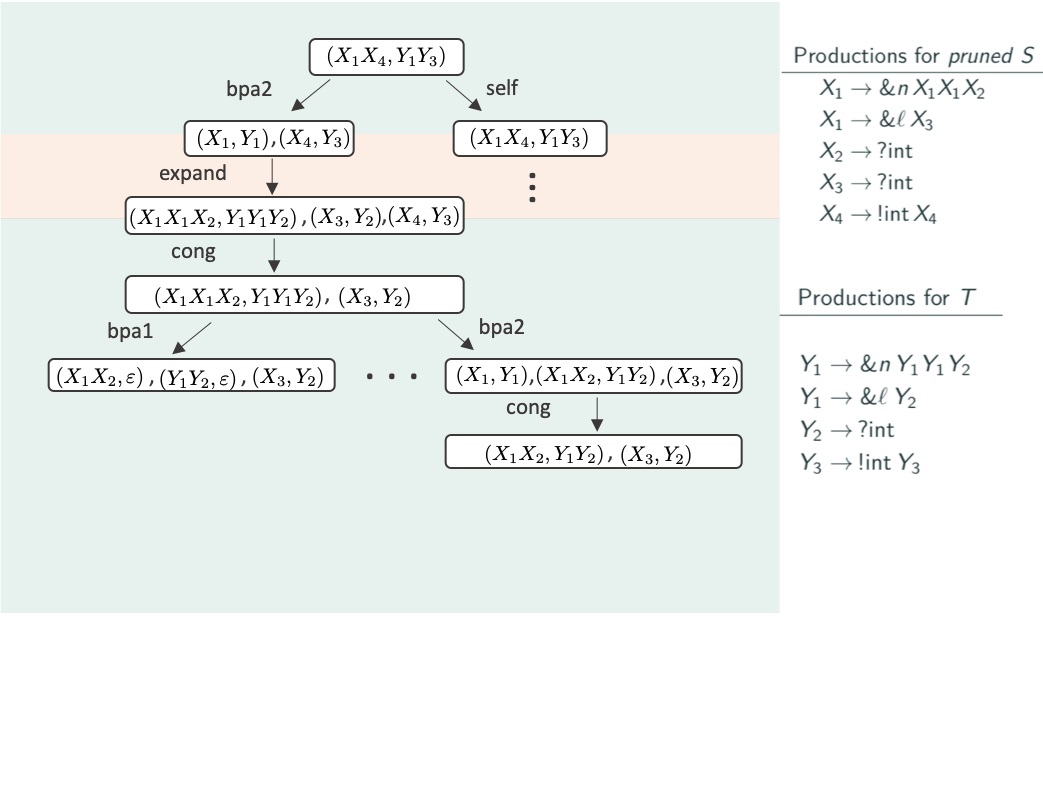
\includegraphics[width=11.5cm]{img/exemplo-4}\smallskip
\end{frame}

\begin{frame}
	\begin{tabular} {l l l }
  		{\color{teal}\rule{3cm}{2pt}} &  $S$ &$\triangleq (\mu x. \&\{n\colon x;x;?\,\intk,
      \ell\colon ?\,\intk \});( \mu z. !\,\intk; z;z )$\\
  		{\color{teal} Example}  &  $T$ &$\triangleq (\mu y. \&\{n\colon y;y,
      \ell\colon \skipk \}; ?\,\intk); (\mu z. !\,\intk; z)$
	\end{tabular}
	\vspace*{2mm}
	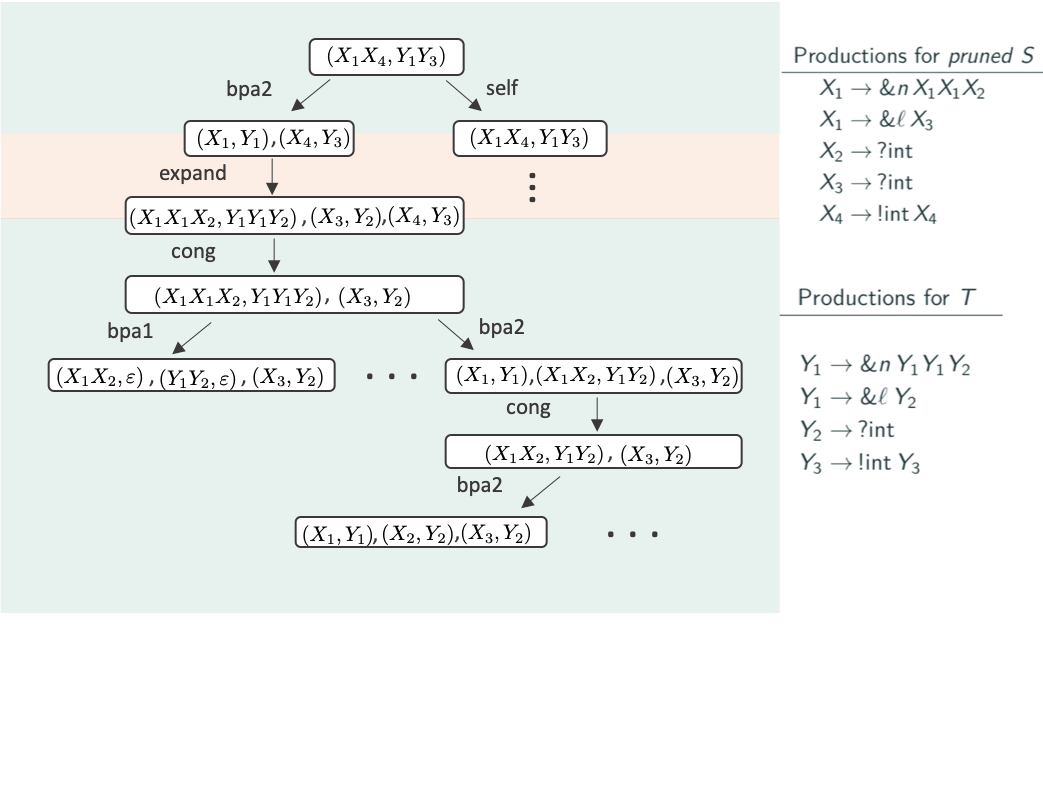
\includegraphics[width=11.5cm]{img/exemplo-3}\smallskip
\end{frame}

\begin{frame}
	\begin{tabular} {l l l }
  		{\color{teal}\rule{3cm}{2pt}} &  $S$ &$\triangleq (\mu x. \&\{n\colon x;x;?\,\intk,
      \ell\colon ?\,\intk \});( \mu z. !\,\intk; z;z )$\\
  		{\color{teal} Example}  &  $T$ &$\triangleq (\mu y. \&\{n\colon y;y,
      \ell\colon \skipk \}; ?\,\intk); (\mu z. !\,\intk; z)$
	\end{tabular}
	\vspace*{2mm}
	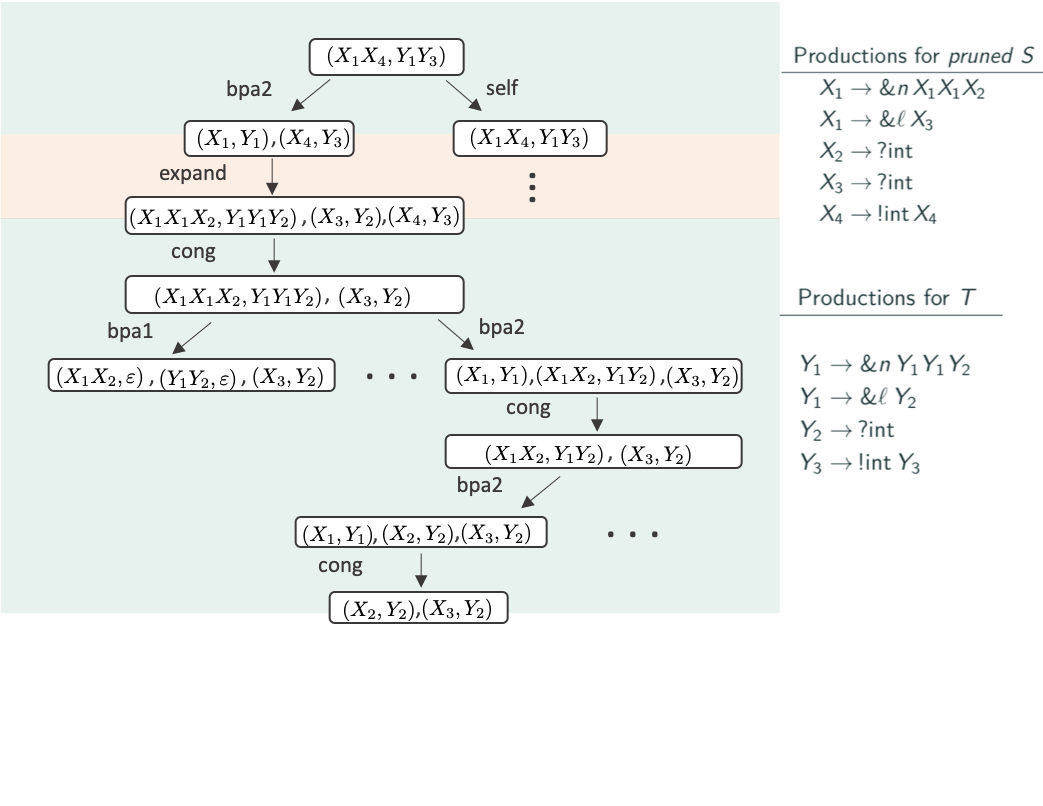
\includegraphics[width=11.5cm]{img/exemplo-2}\smallskip
\end{frame}

\begin{frame}
	\begin{tabular} {l l l }
  		{\color{teal}\rule{3cm}{2pt}} &  $S$ &$\triangleq (\mu x. \&\{n\colon x;x;?\,\intk,
      \ell\colon ?\,\intk \});( \mu z. !\,\intk; z;z )$\\
  		{\color{teal} Example}  &  $T$ &$\triangleq (\mu y. \&\{n\colon y;y,
      \ell\colon \skipk \}; ?\,\intk); (\mu z. !\,\intk; z)$
	\end{tabular}
	\vspace*{2mm}
	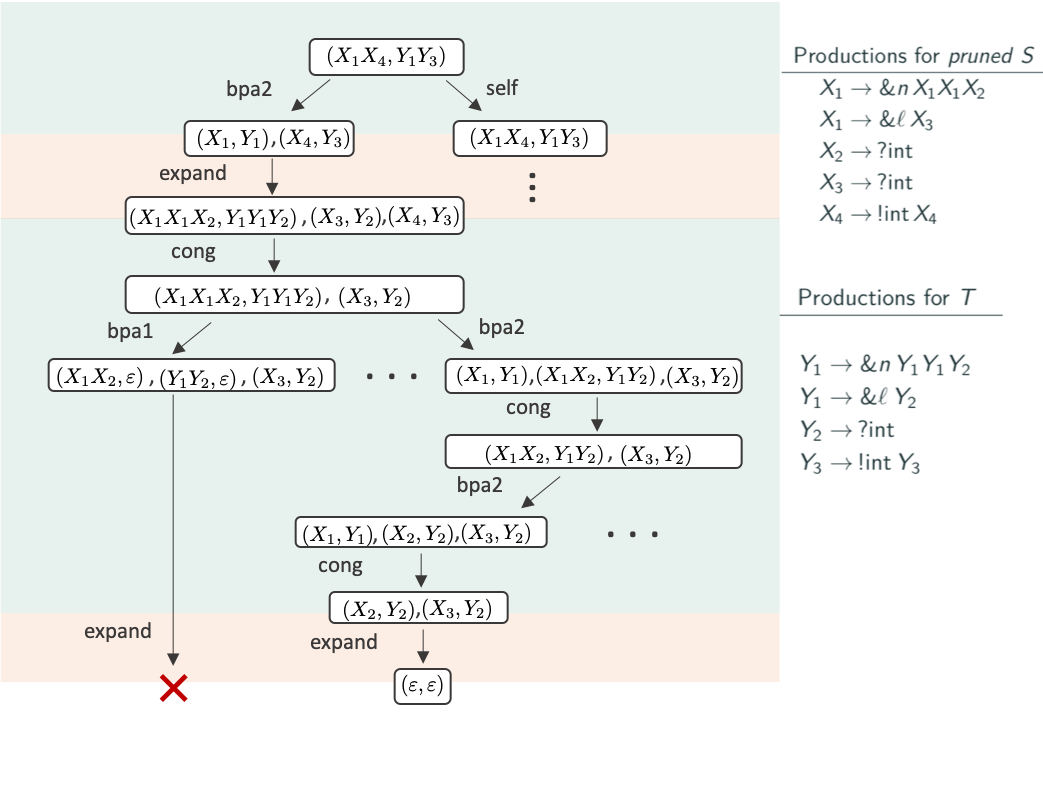
\includegraphics[width=11.5cm]{img/exemplo-1}\smallskip
\end{frame}

\begin{frame}
	\begin{tabular} {l l l }
  		{\color{teal}\rule{3cm}{2pt}} &  $S$ &$\triangleq (\mu x. \&\{n\colon x;x;?\,\intk,
      \ell\colon ?\,\intk \});( \mu z. !\,\intk; z;z )$\\
  		{\color{teal} Example}  &  $T$ &$\triangleq (\mu y. \&\{n\colon y;y,
      \ell\colon \skipk \}; ?\,\intk); (\mu z. !\,\intk; z)$
	\end{tabular}
	\vspace*{2mm}
	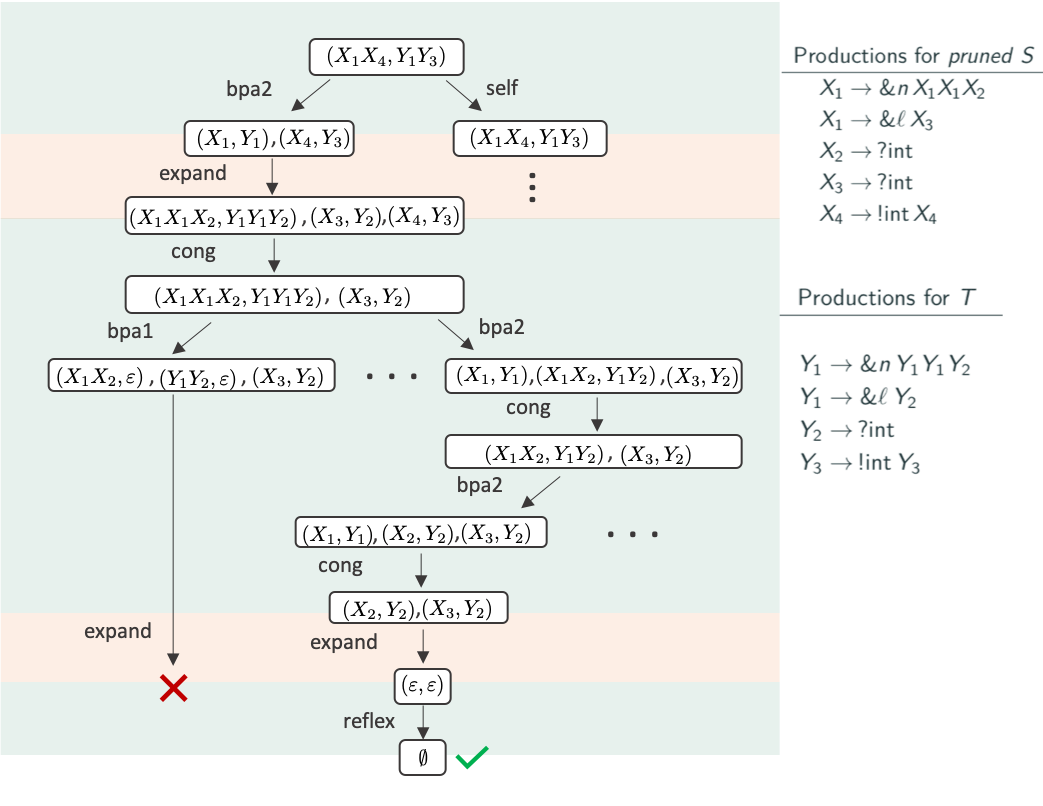
\includegraphics[width=11.5cm]{img/example_expansion_tree}\smallskip
\end{frame}

\begin{frame}{Algorithm for checking the equivalence of CFST \hfill {\color{mLightBrown}Main stages}}
	\begin{center}
		\begin{tikzpicture}[node distance = 2.8cm, auto]
    		% Place nodes
    		\node [block2] (typeToGrammar) {{\bf Convert types to a grammar}\\ 
    		{\color{gray}\texttt{LOHaskellCode $\sim$ 100}}\\
    		Soundness {\color{olive}\checkmark}
    		}; 
    		\node [block2, below=5mm of typeToGrammar] (prune) {{\bf Prune unnormed productions} \\ 
    		{\color{gray}\texttt{LOHaskellCode $\sim$ 30}}\\
    		Soundness {\color{olive}\checkmark} 
    		};
    		\node [block2, below=5mm of prune] (simplifyExpand) {{\bf Simplify and expand}\\ 
    		{\color{gray}\texttt{LOHaskellCode $\sim$ 170}}\\
    		Soundness {\color{olive}\checkmark} 
    		\begin{enumerate}
    			\item The \emph{safeness property ensures soundness}\footnote{Jan{\v{c}}ar, Moller. Techniques for decidability and undecidability of bisimilarity.\\ 1999}
   	 		\end{enumerate}
 			};
    	% Draw edges
    		\path [line] (typeToGrammar) -- (prune);
    		\path [line] (prune) -- (simplifyExpand);
		\end{tikzpicture}
	\end{center}
\end{frame}

\begin{frame}{Evaluation}
  \begin{itemize}
  \item Started with a carefully crafted, manually produced, suite of tests.
  \item They were small, lacking diversity
  \item We went for Automated test generation: QuickCheck
  \item Generating valid (well-formed) types is easy but the probability of
    generating two pairs that turn out to be bisimilar is extremely low.
  \item For this reason, we generate arbitrary pairs of types that are bisimilar
    by construction.
  \end{itemize}
   
%  suite of valid and invalid tests. This test
% suite was assembled by gathering pairs of types that emerged from examples
% we have studied and from programs we have written in FreeST, a programming
% language with context-free session types
  
\end{frame}

\begin{frame}{Generating valid types}
\textbf{Properties of type bisimilarity (a subset)}
  \begin{enumerate} 
    % Congruence 
  \item $\skipk \sim_\types \skipk$ and $\sharp B \sim_\types \sharp B$;
  \item $S;T \sim_\types U;V$ if $S \sim_\types U$ and $T \sim_\types V$;
  \item $\mu X.S \sim_\types \mu X.T$ if $S \sim_\types T$;
  \item $\star\{\ell_i\colon S_i\}_{i\in I}\sim_\types
    \star\{\ell_i\colon T_i\}_{i\in I}$ if $(S_i \sim_\types T_i)_{i\in
      I}$;
    % Laws for sequential composition
  \item $S\sim_\types T;\skipk$ and $S\sim_\types \skipk;T$ if $S \sim_\types T$;
  \item $\star\{\ell_i\colon S_i\}_{i\in I};U\sim_\types
    \star\{\ell_i\colon T_i;V\}_{i\in I}$ if $(S_i \sim_\types T_i)_{i\in
      I}$ and $U \sim_\types V$;
    \item \dots
%  \item $T \sim_\types S$ if $S \sim_\types T$;
%  \item $R;(S;T) \sim_\types (U;V);W$ if $R \sim_\types U$, $S \sim_\types V$, and $T\sim_\types W$;
    % Laws for mu-types
%    $\mu X.\mu Y.S \sim_\types \mu X.\subs XYT \sim_\types \mu Y.\subs
%    YXT$ if $S \sim_\types T$;
%  \item $\mu X.S \sim_\types T$ if $S \sim_\types T$ and $X\notin \mbox{free}(S)$;
%  \item $\subs UXS\sim \subs VXT$  if $S \sim T$ and $U \sim V$;
%  \item $\mu X.S \sim \subs{\mu X.T}{X}T$ if $S \sim T$.
  \end{enumerate}
  
\end{frame}

\begin{frame}
  \frametitle{Generating invalid types}
  For \textbf{non-bisimilar pairs} we add five anti-axioms to the previous list

  \begin{enumerate}
  \item $\skipk \not\sim_\types \sharp B$;
  \item $?B \not\sim_\types !B$;
  \item $\skipk \not\sim_\types \star\{\ell_i\colon S_i\}_{i\in I}$;
  \item $\oplus\{\ell_i\colon S_i\}_{i\in I} \not\sim_\types \&\{\ell_i\colon S_i\}_{i\in I}$;
  \item $\star\{\ell_i\colon S_i\}_{i\in I} \not\sim_\types \star\{\ell_j\colon S_j\}_J$
  \end{enumerate}
\end{frame}

\begin{frame}
  \frametitle{Optimisations}
  The algorithm presented turned out to behave quite poorly
  
  \textbf{We implemented the following optimisations}
  \begin{enumerate}
  \item Eliminating redundant productions in the grammar.
  \item Using a filter rule that removes nodes with hopeless pairs
  \item Using a double-ended queue to prepend promising children
  \end{enumerate}
\end{frame}

\begin{frame}
  \frametitle{Results (I)}
  \begin{itemize}
  \item We tested all the optimisations and their combinations.
  \item Both test suites comprise 2000 entries, featuring types with a number of
    nodes (in the syntax tree) ranging from 1 to 200.
  \item Tests were run under a timeout of 2 minutes.
  \end{itemize}
  \pause
  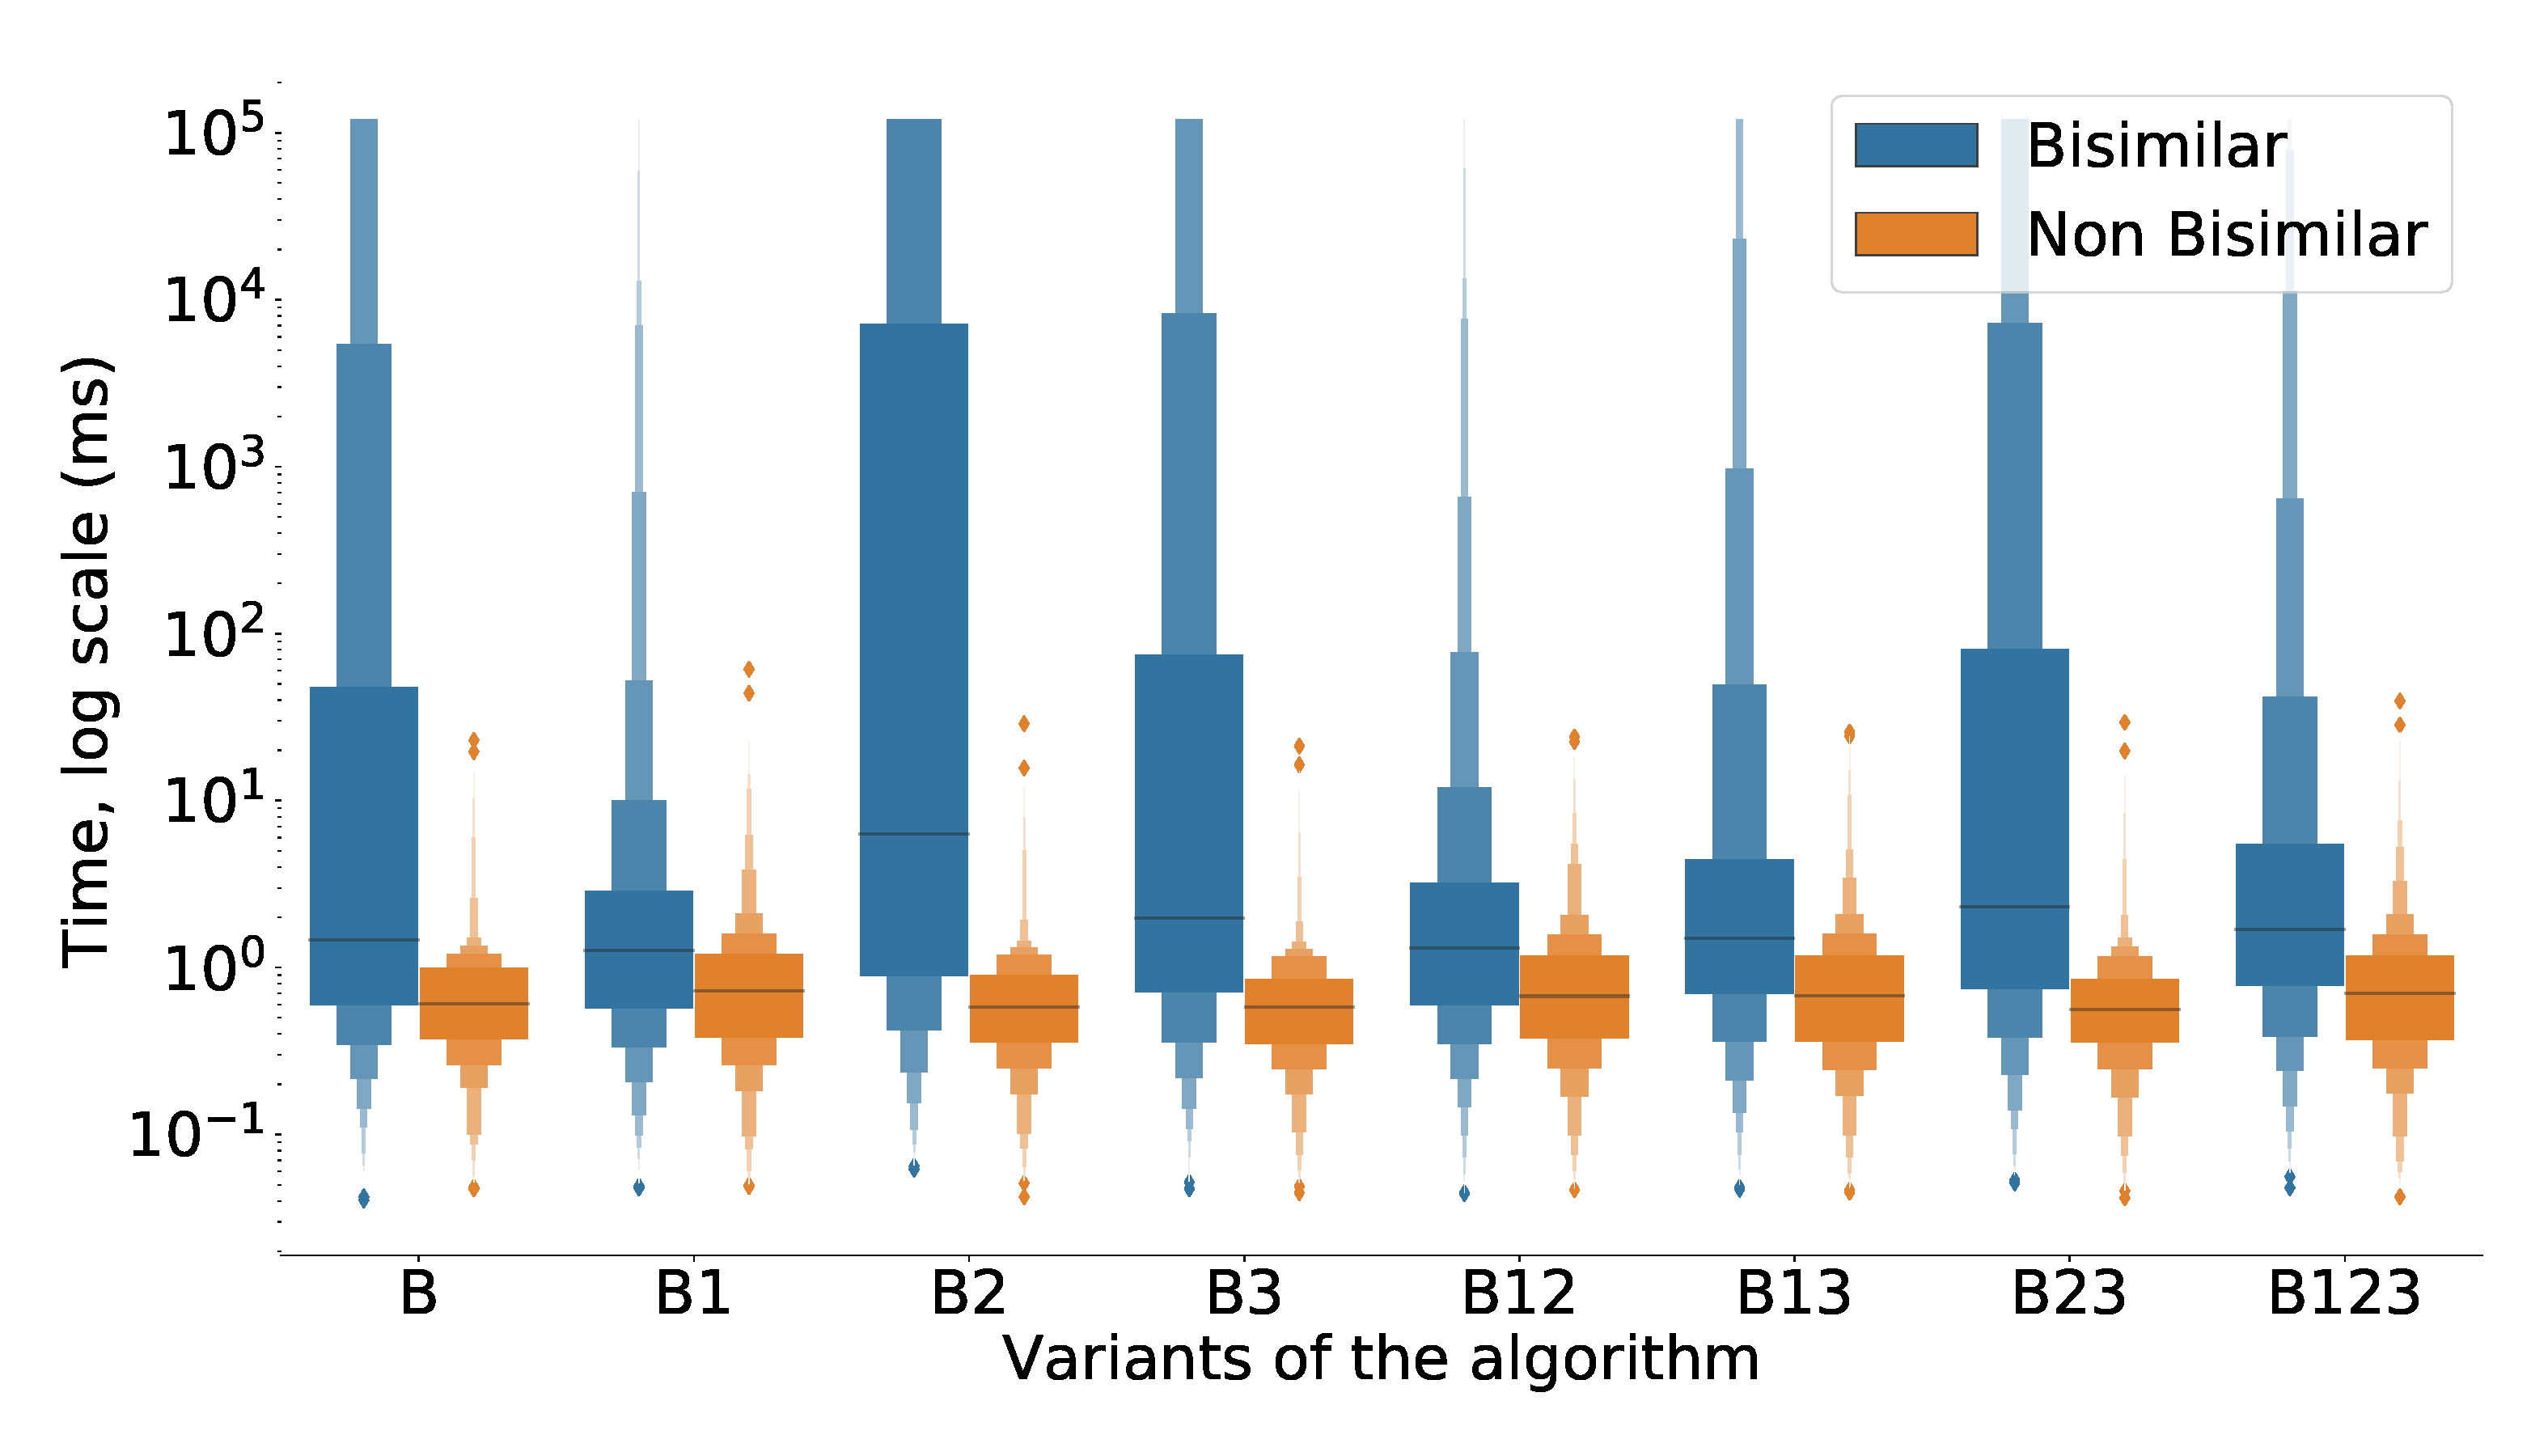
\includegraphics[scale=0.20]{img/distribution_boxplot.pdf}
\end{frame}

\begin{frame}
  \frametitle{Results (II)}
  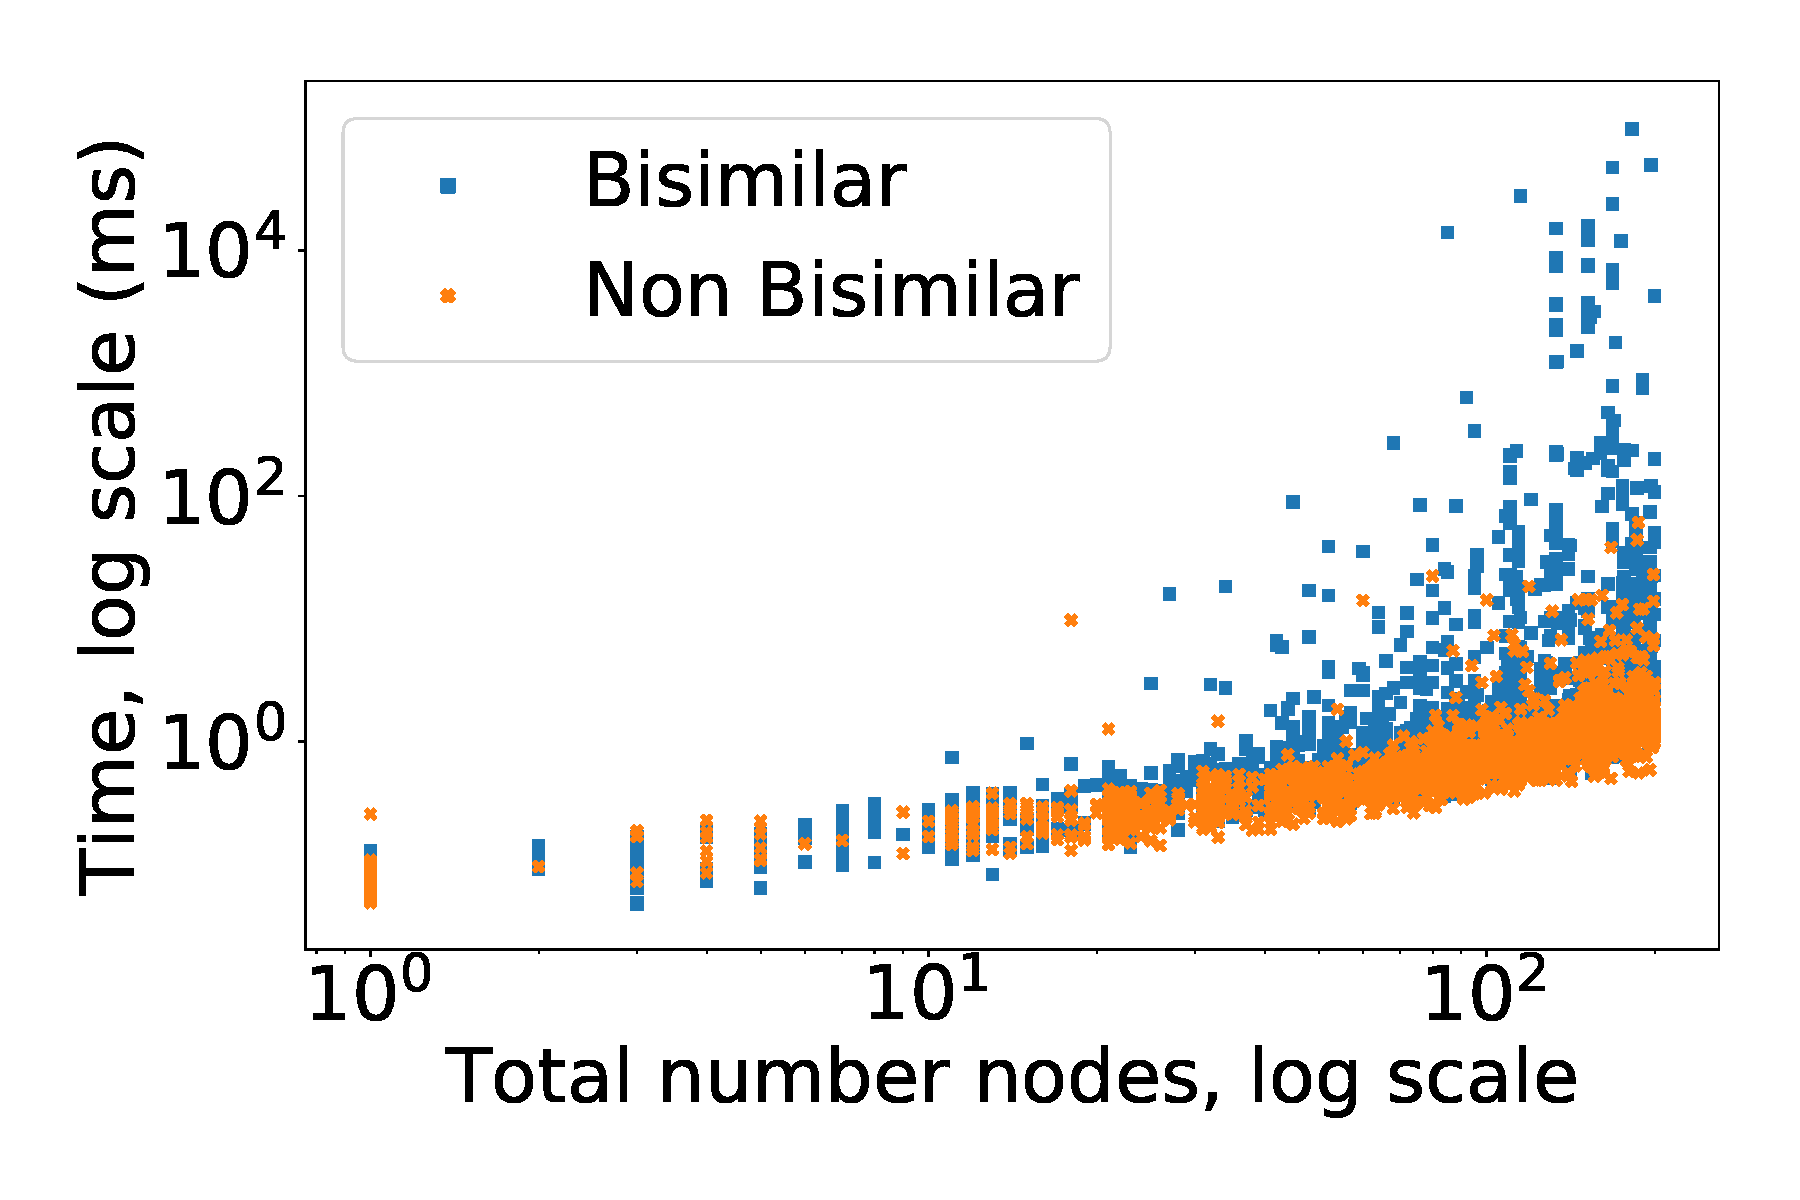
\includegraphics[width=.55\textwidth]{img/nodes_time.pdf}%
  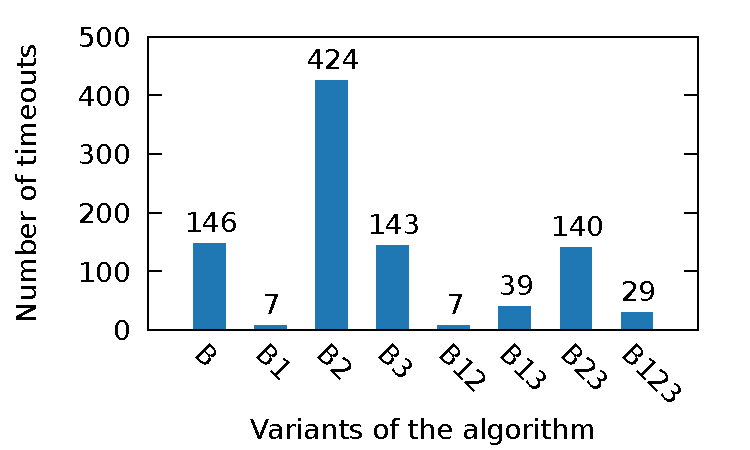
\includegraphics[width=.55\textwidth]{img/timeouts.pdf}
\end{frame}



% \begin{frame}{Implementation strategies}
% 	Implementation choice:
% 	\begin{itemize}
% 		\item Breadth-first search on the tree
% 	\end{itemize}

% 	\pause
% 	Strategic options that can enhance performance:
% 	\begin{itemize}
% 		\item Instead of looking for a fixed point, iterate the simplification phase
% 		\item Apply BPA rules wrapped with blocks of reflexive and congruence rules
% 	\end{itemize}
% 	\pause
% 	We showcase runtimes for four scenarios:
% 	\vspace*{-3mm}

% 	\begin{center}
% 		\begin{tabular}{c | c | c | c | c }
%  			& \multicolumn{2}{c|}{{\color{teal}{\bf Fixed Point Scenario}}} &\multicolumn{2}{c}{{\color{teal}{\hspace*{2mm}\bf Iterated Scenario\hspace*{2mm}}}}\\
%  			& {\enspace\color{mLightBrown}wrapped\enspace} &{\color{mLightBrown}unwrapped}& {\enspace\color{mLightBrown}wrapped\enspace} &{\color{mLightBrown}unwrapped}\\ \hline
%  			{\bf Simplification}& \multicolumn{2}{c |}{find fixed point} & \multicolumn{2}{c}{iterate} \\ \hline
%   			{\bf BPAs wrapped}&$\checkmark$ & $\times$ & $\checkmark$ & $\times$ \\ \hline
% 		\end{tabular}
% 	\end{center}
% \end{frame}

% \begin{frame}{Running times ($\sim$ 150 tests)}
% 	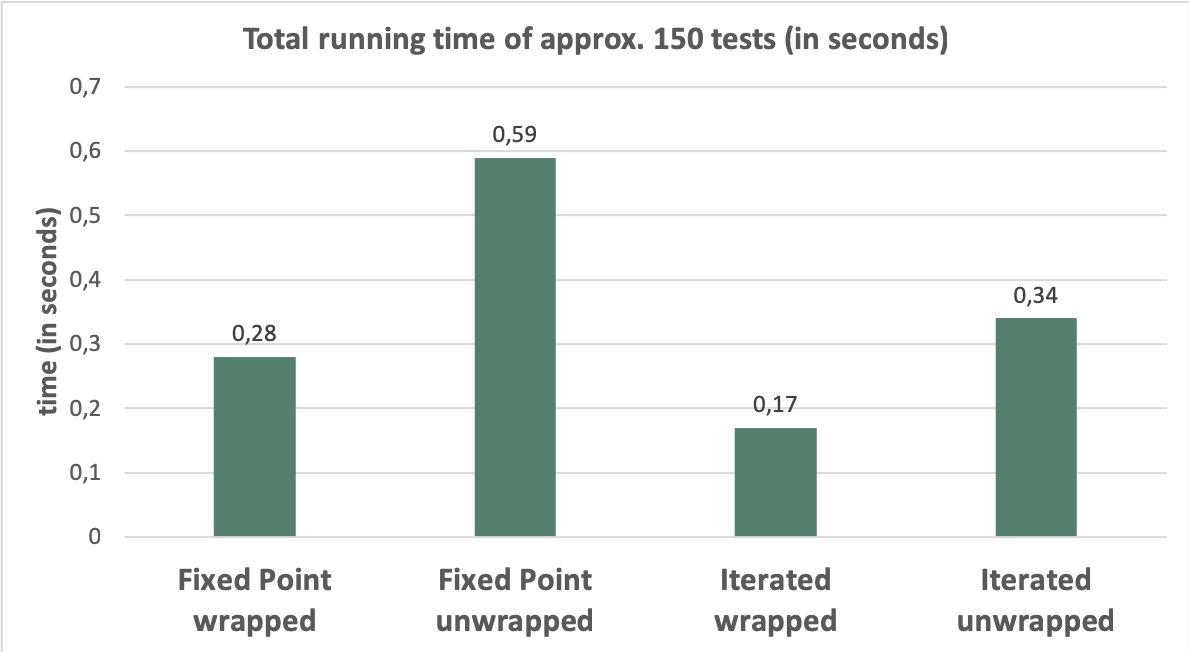
\includegraphics[height=6cm]{img/running_time3}

% 	\fbox{
% 	\begin{tabular}{l l l }
% 		{\small Specs: } & {\small MacBook Air }\\
% 		& {\small 1.8 GHz Intel Core i5} \\
% 		& {\small 8GB of memory}
% 	\end{tabular}}
% \end{frame}

% \begin{frame}{Time and memory allocated \hfill {\color{mLightBrown}Fixed Point}}
% 	\hspace*{-4mm}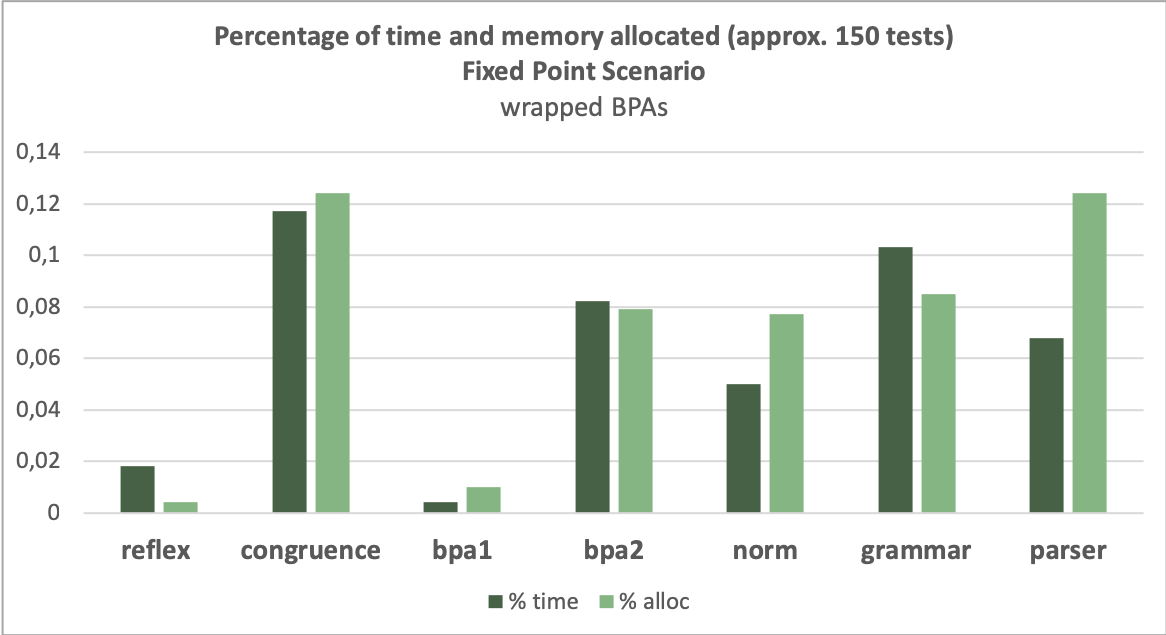
\includegraphics[height=5.8cm]{img/fixed_point2}
% \end{frame}

% %\begin{frame}{Time and memory allocated \hfill {\color{mLightBrown}Iterated }}
% %	\hspace*{-4mm}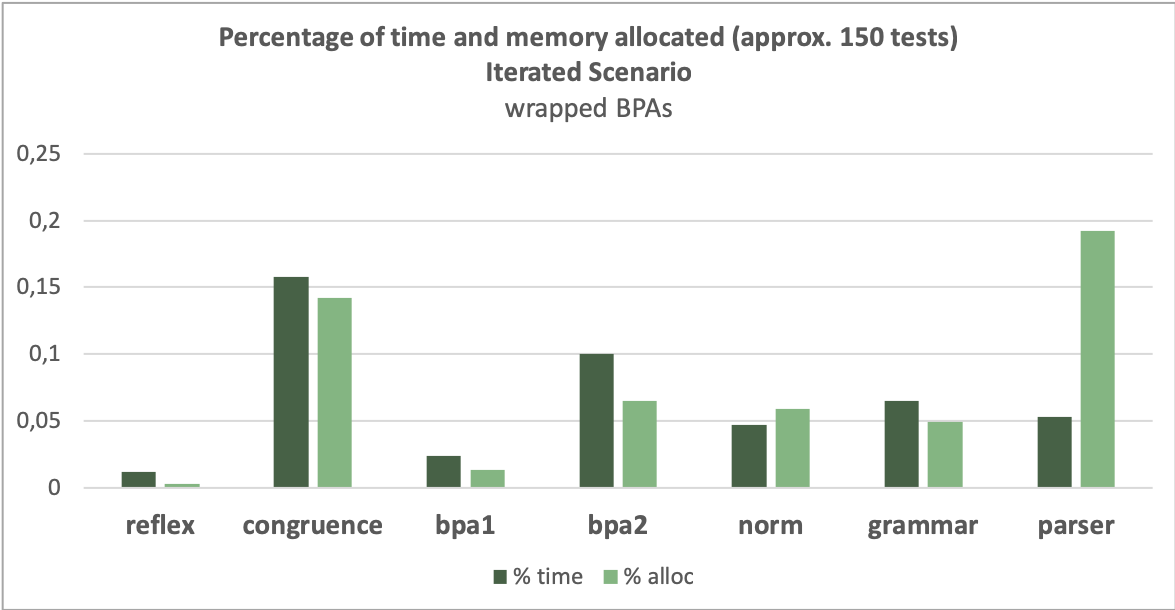
\includegraphics[height=5.8cm]{img/iterated2} 
% %\end{frame}


% \begin{frame}{Towards completeness...}

% 	\metroset{block=fill}
% 	\begin{block}{Finite witness property\footnote{ Christensen et al. Bisimulation equivalence is decidable for all CF processes. 1995}\footnote{Jan{\v{c}}ar, Moller. Techniques for decidability and undecidability of bisimilarity. 1999}}
% 		\smallskip
% 		If $S\sim T$, then there exists a {\bf finite successful branch} in the expansion tree.
% 	\end{block}

% 	\vspace*{5mm}
	
% 	Implementation choices aiming to achieve completeness:
% 	\begin{itemize}
% 		\item Instead of looking for a fixed point, iterate the simplification phase (there may not be a fixed point)
% 		\item Use double ended enqueue, prepending \emph{promising} nodes, as opposed to queuing all new nodes
% 	\end{itemize}
% \end{frame}


% \begin{frame} {Ongoing Work}
% 	\begin{itemize}
% 		\item Soundness {\color{olive}\checkmark}
% 		\item Completeness {\color{orange}?} {\color{gray} ... on our way to achieve it.}
% 		\item Complexity {\color{orange}?} {\color{gray} ... in practice it does not seem to take much longer \\\hspace*{2.4cm} than parsing.}
% 		\item Lines of Haskell code: approx.\ $300$
% 	\end{itemize}
	
% 	{\color{teal}Coming soon: }\\\smallskip
% 	\textsf{FreeST}, a compiler for context-free session types!\\
% 	\hspace*{2cm}{\color{gray}(demos on demand)}
% \end{frame}

\begin{frame}
  \frametitle{Conclusions}

  \begin{itemize}
  \item In order to be incorporate Context-Free session types in programming
    languages and effectively used in compilers, a practical algorithm to decide
    bisimulation is called for.
  \item Taking advantage of a process algebra graph representation of types to
    de- cide bisimulation \footnote{Hirshfeld, Y., Jerrum, M., Moller, F.: A
      polynomial algorithm for deciding bisimilarity of normed context-free
      processes. 1996. }\footnote{Hirshfeld, Y., Moller, F.: A fast algorithm
      for deciding bisimilarity of normed context-free processes. 1994.}, we
    developed one such algorithm and proved it correct.
  \item The algorithm is incorporated in a compiler for a concurrent functional
    language equipped with context-free session types \footnote{Almeida, B.,
      Mordido, A., T. Vasconcelos, V.: Freest: Context-free session types in a
      functional language. 2019}
  \end{itemize}
 \end{frame}




 
\plain{Thank you!}


\end{document}

%%% Local Variables:
%%% mode: latex
%%% TeX-master: t
%%% End:
